\documentclass[11pt]{article}
\usepackage[a4paper, margin=2.5cm]{geometry}
\usepackage{graphicx}
\usepackage{caption}
\usepackage{pdfcomment}
\usepackage{float}
\usepackage{tikz}
\usepackage[polish]{babel}
\usepackage[utf8]{inputenc}
\usepackage[T1]{fontenc}
\captionsetup{font=small, skip=6pt}
\usepackage{titlesec}
\usepackage{parskip}
\setlength{\parskip}{4pt}
\setlength{\textfloatsep}{10pt}
\setlength{\floatsep}{6pt}
\setlength{\intextsep}{10pt}

\titlespacing*{\section}{0pt}{2ex plus .2ex minus .2ex}{1ex plus .2ex}
\titlespacing*{\subsection}{0pt}{1ex plus .1ex minus .1ex}{0.5ex plus .1ex}

    
\usepackage{parskip}
\setlength{\parskip}{2pt}

\title{Wzmacniacze mocy w napędzie elektrycznym. Przekształtnik tranzystorowy i tyrystorowy.}

\author{
  Mateusz Jaworski \\
  Piotr Migdalek \\
  Pawel Michalski \\
  Jakub Jaszczak \\
  Franciszek Janicki
}

\begin{document}

\maketitle

\section{Część I}

\subsection{WZMACNIACZ LINIOWY / WZMACNIACZ IMPULSOWY}

a) Badanie sprawnosci wzmacniacza liniowego BJT

Zbadano moc na wejsciu i wyjsciu wzmacniacza liniowego w technologii BJT.\\

\begin{figure}[H]
\centering
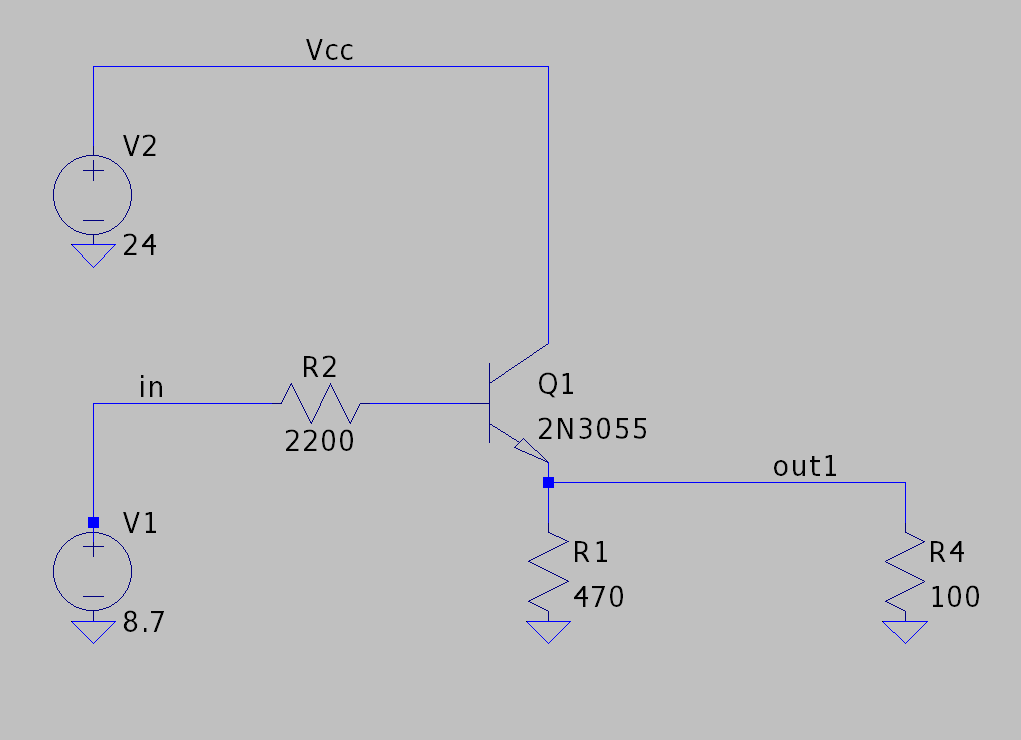
\includegraphics[width=0.8\textwidth]{aun1_liniowy_bjt.png}
\caption{Schemat pomiarowy wzmacniacza liniowego BJT}
\end{figure}

\begin{table}[H]
\centering
\begin{tabular}{|c|c|c|c|c|}
\hline
\textbf{Vcc [V]} & \textbf{V\_in [V]} & \textbf{P\_in + P\_vcc [mW]} & \textbf{P\_out [W]} & \textbf{Sprawność [\%]} \\
\hline
24 & 2  & 0{,}667  & 0{,}014683 & 2{,}201 \\
\hline
24 & 4  & 1{,}525  & 0{,}070000 & 4{,}590 \\
\hline
24 & 6  & 2{,}380  & 0{,}166000 & 6{,}975 \\
\hline
24 & 8  & 3{,}242  & 0{,}360000 & 11{,}104 \\
\hline
24 & 10 & 4{,}097  & 0{,}477000 & 11{,}643 \\
\hline
24 & 12 & 4{,}950  & 0{,}690000 & 13{,}939 \\
\hline
24 & 14 & 5{,}800  & 0{,}941000 & 16{,}224 \\
\hline
24 & 16 & 6{,}640  & 1{,}220000 & 18{,}373 \\
\hline
24 & 18 & 7{,}490  & 1{,}540000 & 20{,}561 \\
\hline
24 & 20 & 8{,}330  & 1{,}940000 & 23{,}289 \\
\hline
\end{tabular}
\caption{Sprawnosc pracy wzmacniacza liniowego BJT}
\end{table}

Jak widzimy sprawnosc jest bardzo mala. Wynika to z faktu, ze tranzystor nie wysterowuje sie calkowicie,
czesc energii przeksztalcana jest na cieplo.

b) Badanie sprawnosci wzmacniacza impulsowego BJT, porownanie z wzmacniaczem liniowym BJT

Zbadano moc na wejsciu i wyjsciu wzmacniacza impulsowego w technologii BJT.\\

\begin{figure}[H]
\centering
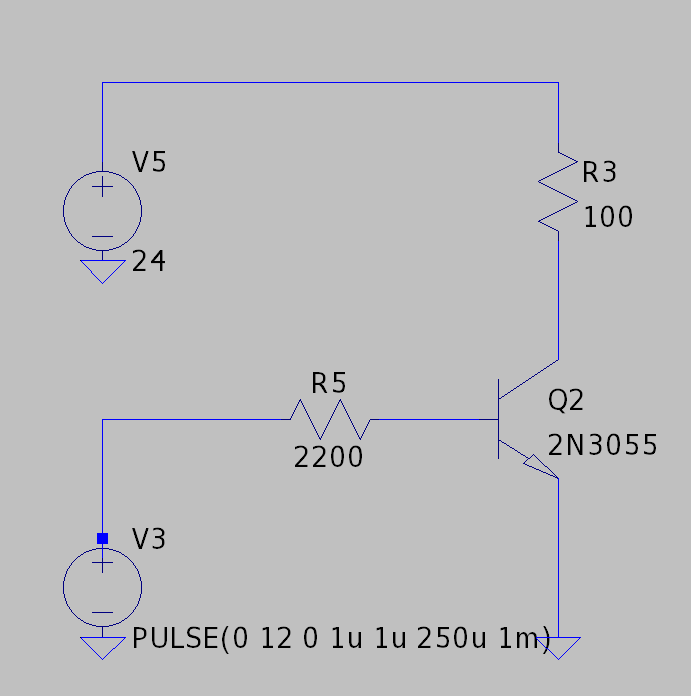
\includegraphics[width=0.8\textwidth]{aun1_impulsowy_bjt.png}
\caption{Schemat pomiarowy wzmacniacza impulsowego BJT}
\end{figure}

\begin{table}[H]
\centering
\begin{tabular}{|c|c|c|c|c|}
\hline
\textbf{Vcc [V]} & \textbf{V\_in [V]} & \textbf{P\_vcc + P\_in [W]} & \textbf{P\_out [W]} & \textbf{Sprawność [\%]} \\
\hline
24 & 2  & 0{,}54825 & 0{,}499   & 91{,}017 \\
\hline
24 & 4  & 1{,}054   & 0{,}974   & 92{,}410 \\
\hline
24 & 6  & 1{,}549   & 1{,}453   & 93{,}802 \\
\hline
24 & 8  & 2{,}046   & 1{,}928   & 94{,}233 \\
\hline
24 & 10 & 2{,}544   & 2{,}4023  & 94{,}430 \\
\hline
24 & 12 & 3{,}0476  & 2{,}882   & 94{,}566 \\
\hline
24 & 14 & 3{,}545   & 3{,}356   & 94{,}669 \\
\hline
24 & 16 & 4{,}042   & 3{,}831   & 94{,}780 \\
\hline
24 & 18 & 4{,}546   & 4{,}311   & 94{,}831 \\
\hline
24 & 20 & 5{,}043   & 4{,}833   & 95{,}836 \\
\hline
\end{tabular}
\caption{Sprawnosc pracy wzmacniacza impulsowego BJT}
\end{table}

Jak widzimy, sprawnosc jest bardzo duza, wynika to z faktu, ze wzmacniacz impulsowy dziala tylko w 2 stanach tranzystora:
zaporowym oraz przewodzenia, gdzie kiedy klucz jest rozlaczony, nie ma strat, w momencie przewodzenia straty sa minimalne. Przy duzych czestotliwosciach przelaczania glowne zrodlo strat to straty laczeniowe, ktore mozemy minimalizowac dobierajac tranzystor o odpowiednich parametrach.\\

Porownano sprawnosci wzmacniaczy liniowego oraz impulsowego w technologii BJT.\\

\begin{figure}[H]
\centering
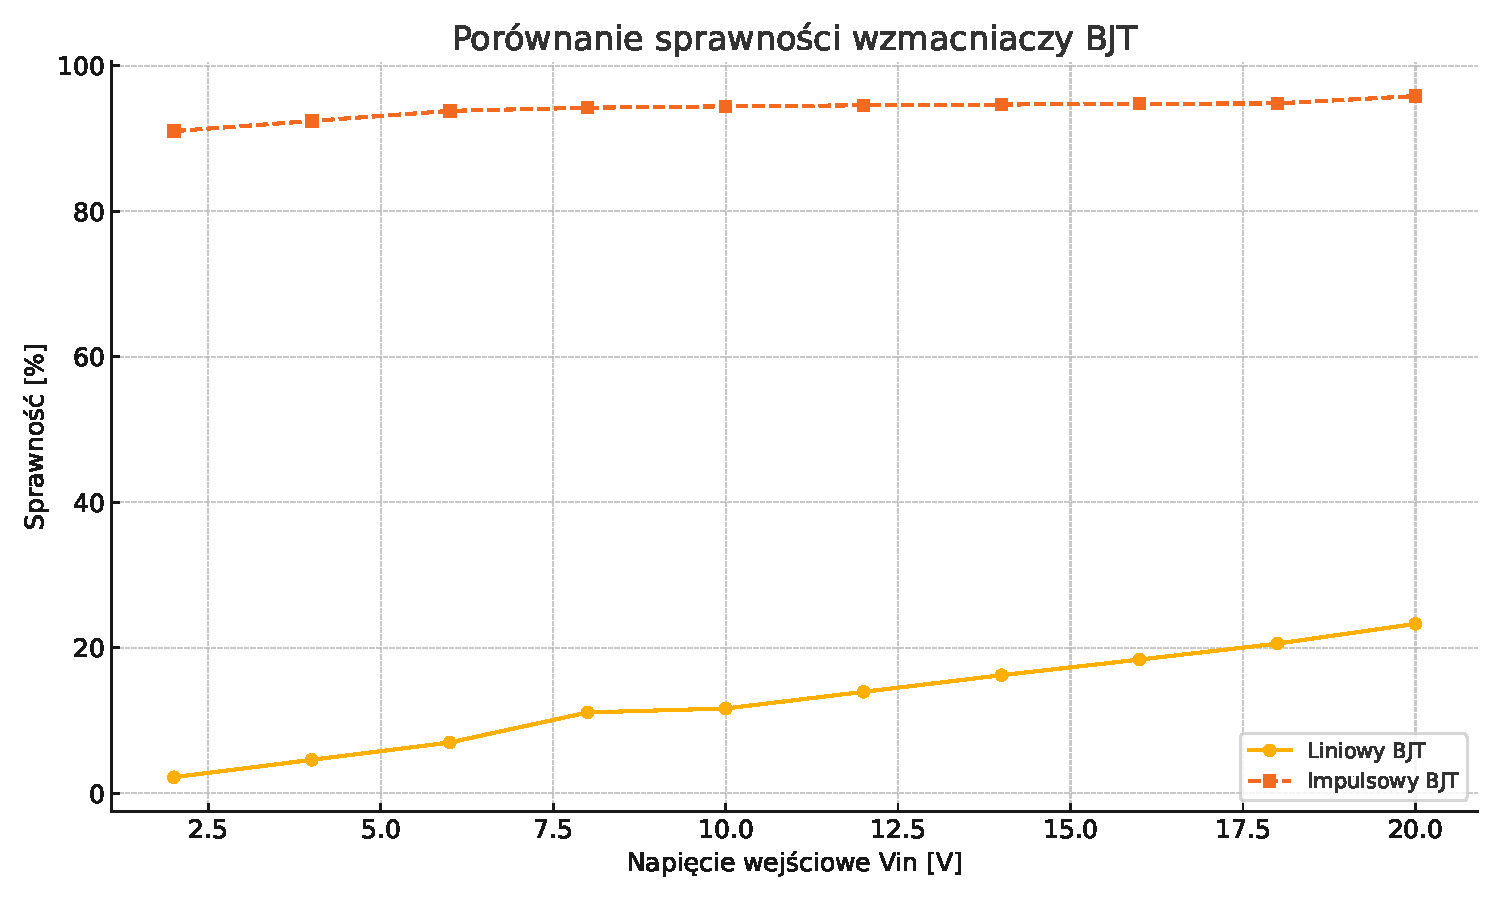
\includegraphics[width=0.8\textwidth]{aun1_liniowy_impulsowy_bjt.pdf}
\caption{Wykres sprawnosci wzmacniacza liniowego i impulsowego BJT}
\end{figure}

Jak widzimy, w obydwu przypadkach sprawnosc rosnie wraz ze zblizaniem sie napiecia sredniego na tranzystorze do napiecia zasilania. Wzmacniacz impulsowy ktory zachowuje bardzo duza sprawnosc dla calego zakresu napiecia ma znaczaca przewage,
wykorzystuje bowiem jedynie stan przewodzenia i zaporowy, a jedyne znaczace straty to straty laczeniowe
(straty przewodzenia odgrywaja duza role tylko przy nizszych czestotliwosciach).\\

\subsection{TECHNOLOGIA BJT/MOSFET}

c) Badanie sprawności wzmacniacza impulsowego MOSFET i porównanie z wzmacniaczem impulsowym BJT oraz porównanie wpływu Rds_on i ładunku bramki na sprawność

Zbadano moc na wejsciu i wyjsciu wzmacniacza impulsowego w technologiach BJT i MOSFET.\\

\begin{figure}[H]
\centering
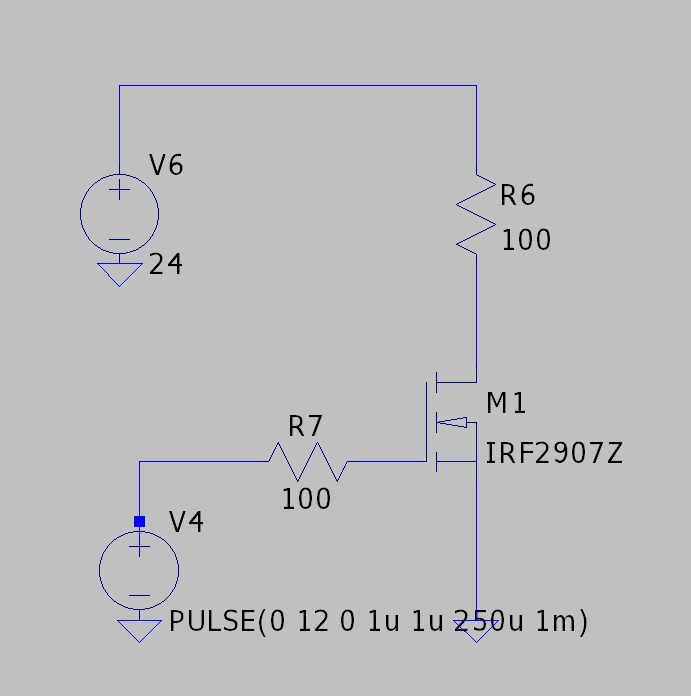
\includegraphics[width=0.8\textwidth]{aun1_impulsowy_mosfet.png}
\caption{Schemat pomiarowy wzmacniacza impulsowego MOSFET}
\end{figure}

\begin{table}[H]
\centering
\begin{tabular}{|c|c|c|c|c|}
\hline
\textbf{Vcc [V]} & \textbf{V\_in [V]} & \textbf{P\_vcc + P\_in [mW]} & \textbf{P\_out [W]} & \textbf{Sprawność [\%]} \\
\hline
24 & 2  & 0{,}499    & 0{,}4956   & 99{,}319 \\
\hline
24 & 4  & 0{,}95412  & 0{,}9506   & 99{,}631 \\
\hline
24 & 6  & 1{,}461    & 1{,}4575   & 99{,}760 \\
\hline
24 & 8  & 1{,}939    & 1{,}9355   & 99{,}819 \\
\hline
24 & 10 & 2{,}417    & 2{,}4135   & 99{,}855 \\
\hline
24 & 12 & 2{,}9009   & 2{,}8974   & 99{,}879 \\
\hline
24 & 14 & 3{,}379    & 3{,}375    & 99{,}882 \\
\hline
24 & 16 & 3{,}857    & 3{,}853    & 99{,}896 \\
\hline
24 & 18 & 4{,}3409   & 4{,}3373   & 99{,}917 \\
\hline
24 & 20 & 5{,}760    & 5{,}759    & 99{,}983 \\
\hline
\end{tabular}
\caption{Sprawnosc pracy wzmacniacza impulsowego MOSFET}
\end{table}

\begin{figure}[H]
\centering
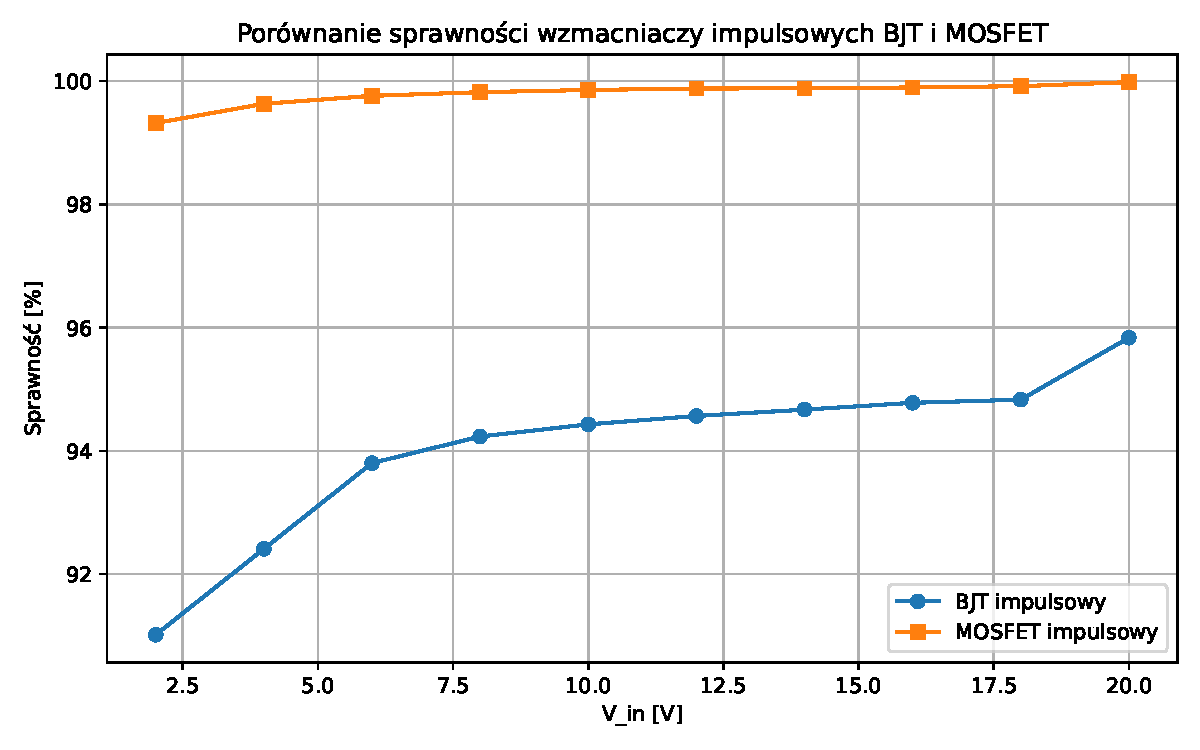
\includegraphics[width=0.8\textwidth]{aun1_imp_bjt_vs_mosfet.pdf}
\caption{Wykres sprawnosci wzmacniacza impulsowego BJT i MOSFET}
\end{figure}

Jak widzimy, tranzystor MOSFET charakteryzuje sie wieksza sprawnoscia anizeli BJT.\\

Zbadano wplyw parametrow Rds\_on oraz GateCharge w tranzystorach MOSFET
na sprawnosc wzmacniacza impulsowego. \\ 

\begin{table}[H]
\centering
\begin{tabular}{|c|c|c|}
\hline
\textbf{Parametr} & \textbf{IRFL4310} & \textbf{IRF2907Z} \\
\hline
Rds\_on & 200\,m\(\Omega\) & 3,5\,m\(\Omega\) \\
\hline
GateCharge & 28\,nC & 180\,nC \\
\hline
\end{tabular}

\caption{Porównanie parametrów tranzystorów IRFL4310 i IRF2907Z}
\end{table}

\begin{table}[H]
\centering
\begin{tabular}{|c|c|c|c|c|c|c|}
\hline
\textbf{f [Hz]} & \multicolumn{3}{c|}{\textbf{IRFL4310}} & \multicolumn{3}{c|}{\textbf{IRF2907Z}} \\
\cline{2-7}
 & $P_{in}+P_{vcc}$ [W] & $P_{out}$ [W] & Sprawność [\%] & $P_{in}+P_{vcc}$ [W] & $P_{out}$ [W] & Sprawność [\%] \\
\hline
1k   & 2,9009 & 2,8836 & 99,41 & 2,9009 & 2,8988 & 99,93 \\
\hline
2k   & 2,8917 & 2,8916 & 99,99 & 2,9219 & 2,9177 & 99,85 \\
\hline
4k   & 2,9078 & 2,9076 & 99,99 & 2,9638 & 2,9555 & 99,72 \\
\hline
8k   & 2,9400 & 2,9397 & 99,96 & 3,0478 & 3,0312 & 99,45 \\
\hline
16k  & 3,1335 & 3,1321 & 99,96 & --- & -- & --- \\
\hline
32k  & 3,1332 & 3,1319 & 99,92 & --- & --- & --- \\
\hline
64k  & 3,3909 & 3,3882 & 99,92 & --- & --- & --- \\
\hline
\end{tabular}
\caption{Porównanie sprawności tranzystorów IRFL4310 oraz IRF2907Z przy 50\% duty cycle.}
\end{table}

Jak widzimy, dla częstotliwości PWM powyżej 64\,kHz tranzystor \textbf{IRFL4310} (o większym $R_{\text{DS(on)}}$) zaczyna nie nadążać z szybkim otwieraniem i zamykaniem, natomiast już przy 16\,kHz ograniczeniem staje się tranzystor \textbf{IRF2907Z}, posiadający duży ładunek bramki ($Q_g$).
Dobór odpowiedniego tranzystora pod kątem energooszczędności to kompromis między tymi dwoma parametrami: rezystancją $R_{\text{DS(on)}}$ a ładunkiem bramki $Q_g$.
Spowodowane jest to faktem, że \textbf{straty przewodzenia} dominują przy niskich częstotliwościach i dużych prądach, a ich wartość określa wzór:
\[
P_{\text{ON}} = I^2 \cdot R_{\text{DS(on)}}
\]
Natomiast przy wysokich częstotliwościach PWM dominują \textbf{straty przełączania}, które w przybliżeniu można traktowac jako proporcjonalne do ladunku bramki.
Dlatego wybór tranzystora należy zawsze dostosować do konkretnej częstotliwości pracy i charakterystyki obciążenia.\\

\begin{figure}[H]
\centering
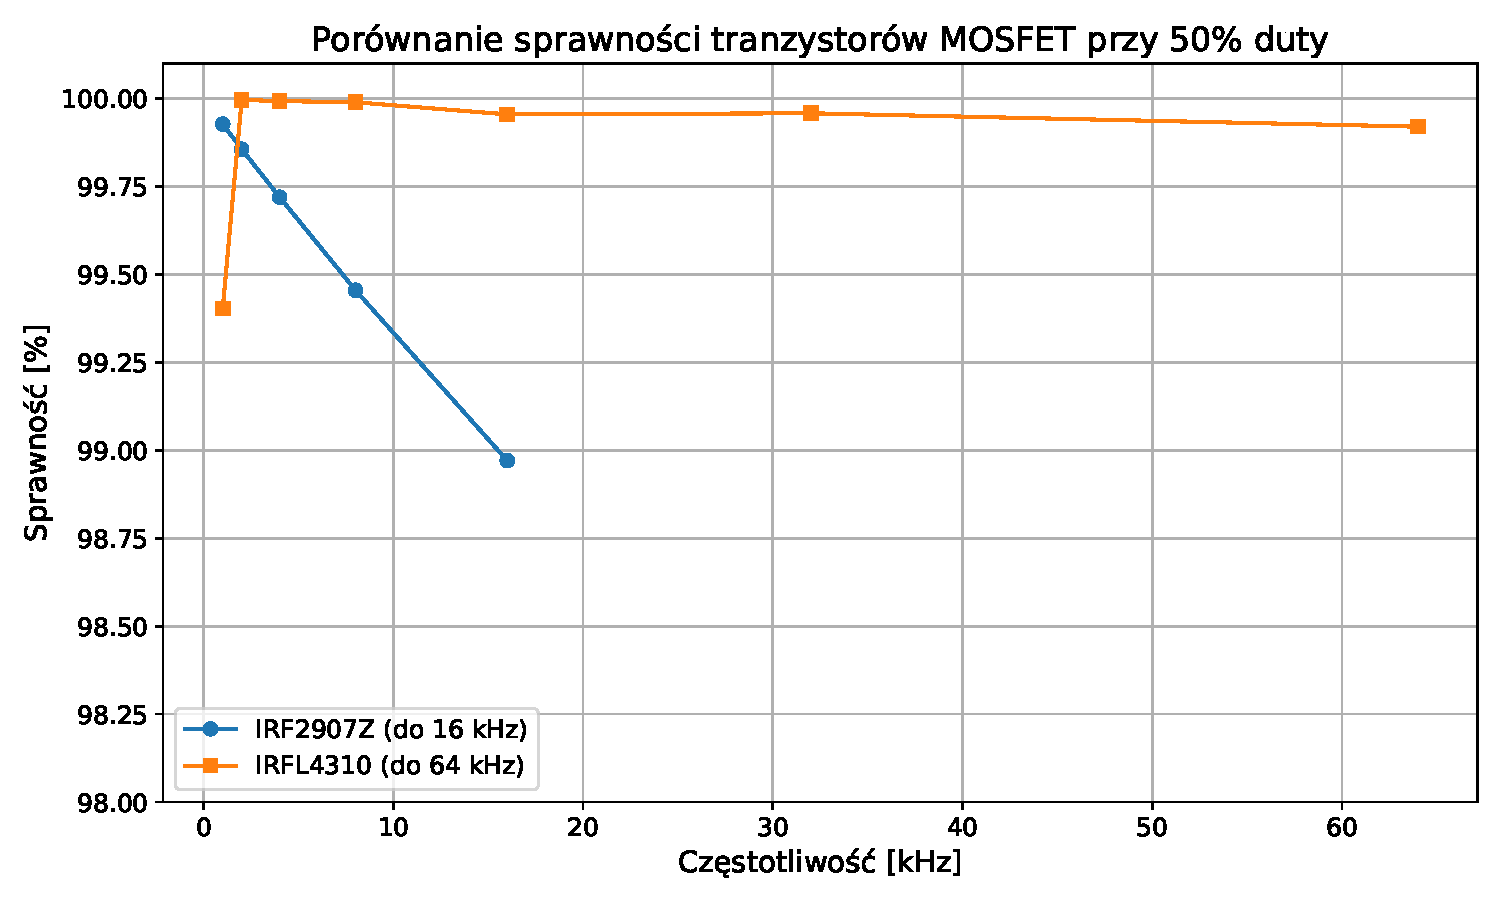
\includegraphics[width=0.8\textwidth]{aun1_imp_mosfet_comparison.pdf}
\caption{Wykres sprawnosci wzmacniaczy impulsowych MOSFET}
\end{figure}

Jak widzimy, tranzystor IRFL4310 o mniejszym ladunku bramki cechuje sie wieksza sprawnoscia przy wiekszych czestotliwosciach (oraz jest w stanie w ogole poprawnie przy nich pracowac), natomiast tranzystor IRF2907Z
cechuje sie wieksza sprawnosciia dla mniejszych czestotliwosci, co czyni go lepszym wyborem dla zastosowan, gdzie
straty przewodzenia stanowia glowny problem.\\

\subsection{ZJAWISKA W OBWODZIE D-S TRANZYSTORA WYNIKAJĄCE Z PARAMETRÓW PASOŻYTNICZYCH OBWODU}

d) Badanie wartosci pasozytniczych w ukladzie RLD sterowanym tranzystorem MOSFET

\begin{figure}[H]
\centering
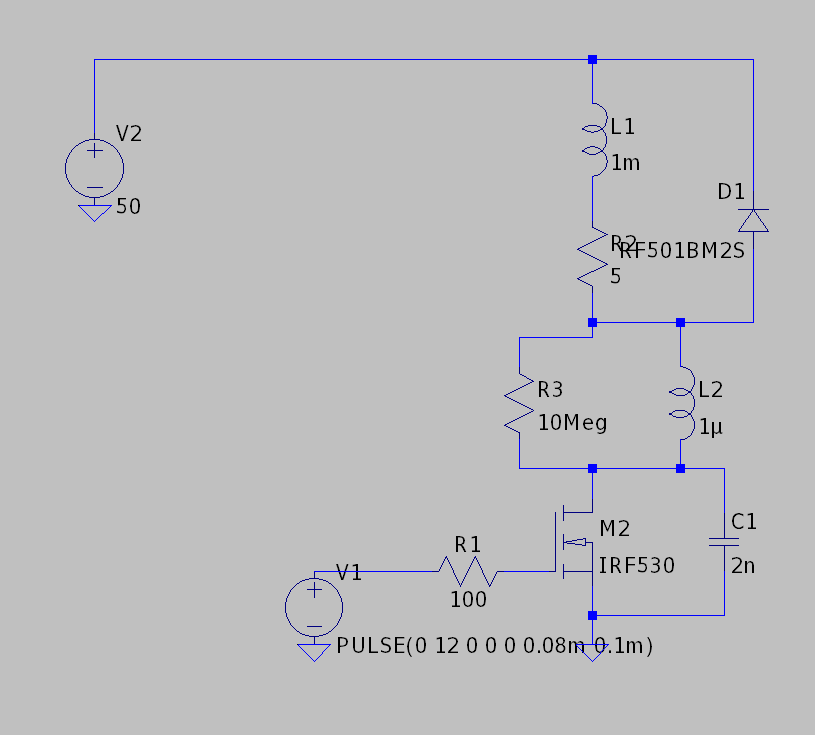
\includegraphics[width=0.8\textwidth]{aun1_rld_without_snubber.png}
\caption{Schemat pomiarowy ukladu RLD sterowanego tranzystorem MOSFET}
\end{figure}

\begin{figure}[H]
\centering
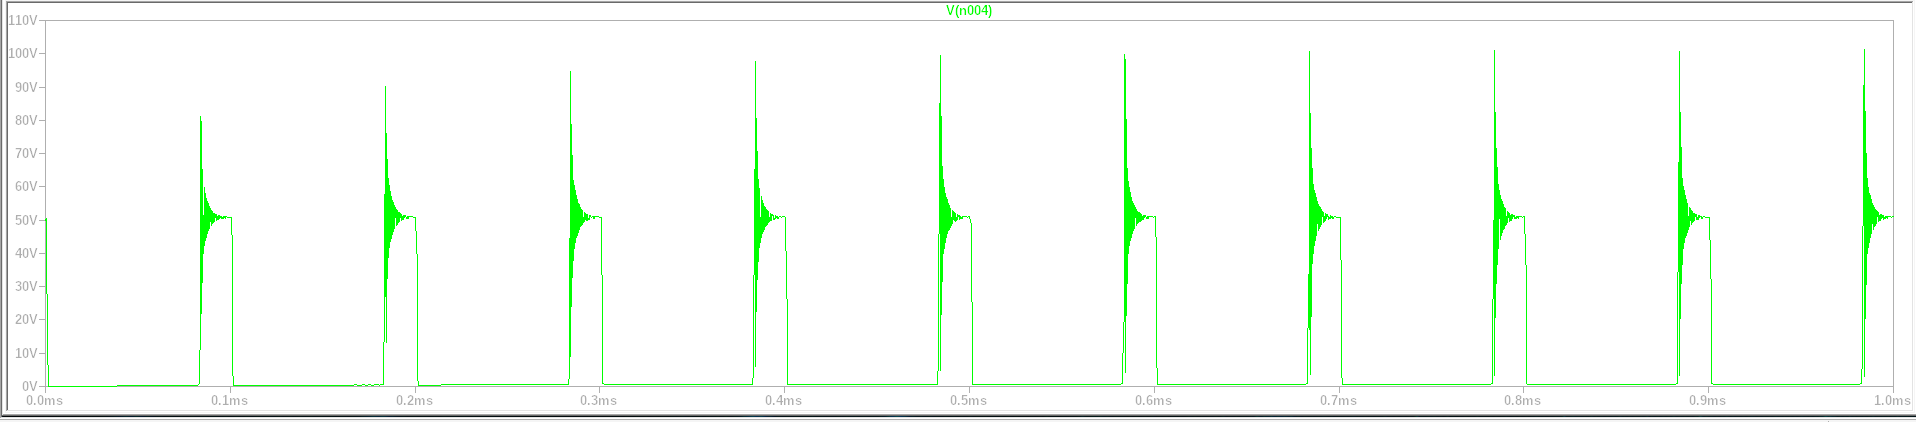
\includegraphics[width=0.8\textwidth]{aun1_rld_without_snubber_rgate100ohm.png}
\caption{Przebieg napiecia na wyjsciu tranzystora MOSFET sterujacego ukladem RLD z rezystancja bramki 100 [\Omega]}
\end{figure}

\begin{figure}[H]
\centering
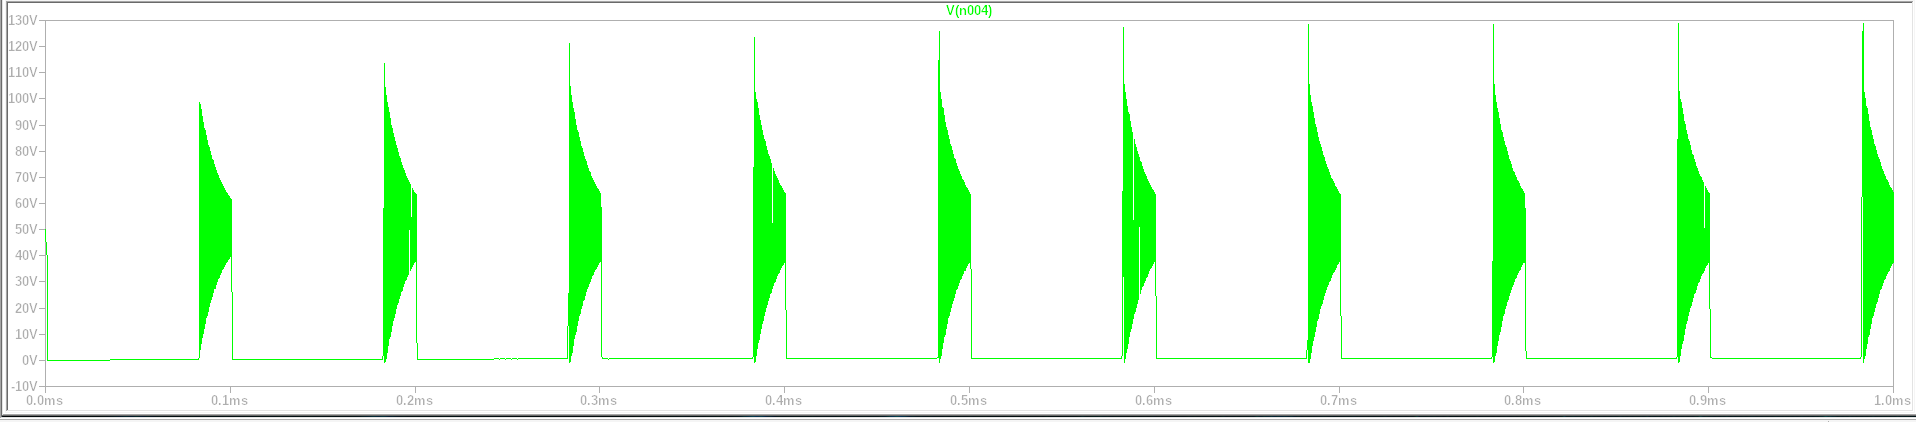
\includegraphics[width=0.8\textwidth]{aun1_rld_without_snubber_rgate10ohm.png}
\caption{Przebieg napiecia na wyjsciu tranzystora MOSFET sterujacego ukladem RLD z rezystancja bramki 10 [\Omega]}
\end{figure}

e) Dobor tlumika oscylacji napiecia (parametry snubber'a)

\begin{figure}[H]
\centering
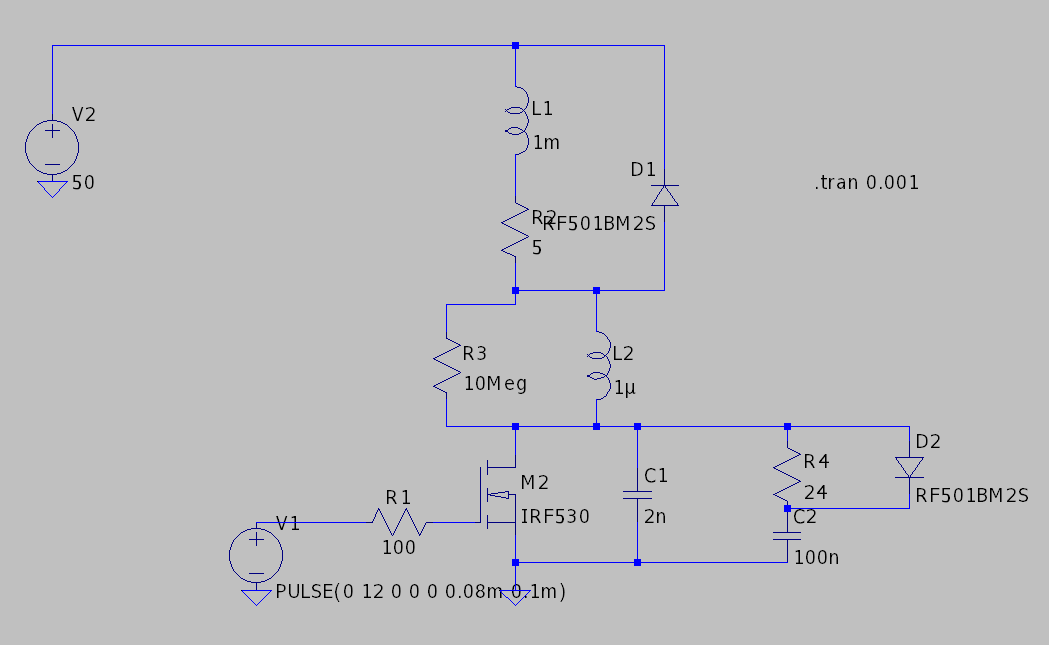
\includegraphics[width=0.8\textwidth]{aun1_rld_with_snubber.png}
\caption{Schemat pomiarowy ukladu RLD sterowanego tranzystorem MOSFET z tlumikiem oscylacji w obwodzie D-S tranzystora}
\end{figure}

Dobór parametrów tłumika (snubbera):
\begin{enumerate}
  \item Mierzymy częstotliwość oscylacji:
  \[
  f_0 = \SI{3.3}{\mega\hertz}
  \]
  \item Dobieramy kondensator o pojemności większej niż pojemność pasożytnicza tranzystora i mierzymy nową częstotliwość zakłóceń:
  \[
  C_1 = \SI{1}{\nano\farad}, \quad f_1 = \SI{2.7}{\mega\hertz}
  \]
  \item Liczymy stosunek częstotliwości:
  \[
  m = \frac{f_0}{f_1} = \frac{3.3}{2.7} = 1.22
  \]
  \item Obliczamy pojemność pasożytniczą tranzystora:
  \[
  C_0 = \frac{C_1}{m^2 - 1} = \frac{1\,\text{nF}}{1.22^2 - 1} = \SI{2.02}{\nano\farad}
  \]
  \item Obliczamy wartość indukcyjności pasożytniczej:
  \[
  L_0 = \frac{(m^2 - 1)}{(2\pi f_0)^2 C_1} = \frac{(1.22^2 - 1)}{(2\pi \cdot 3.3 \times 10^6)^2 \cdot 1 \times 10^{-9}} = \SI{1.15}{\micro\henry}
  \]
  \item Obliczamy minimalną wartość pojemności kondensatora snubbera:
  \[
  C_{\text{snubber}} = 3C_0 = 3 \cdot \SI{2.02}{\nano\farad} = \SI{6.06}{\nano\farad}
  \]
  \item Obliczamy wartość rezystancji w snubberze:
  \[
  R_{\text{snubber}} = \sqrt{\frac{L_0}{C_0}} = \sqrt{\frac{1.15 \times 10^{-6}}{2.02 \times 10^{-9}}} = \SI{24}{\ohm}
  \]
\end{enumerate}

\begin{figure}[H]
\centering
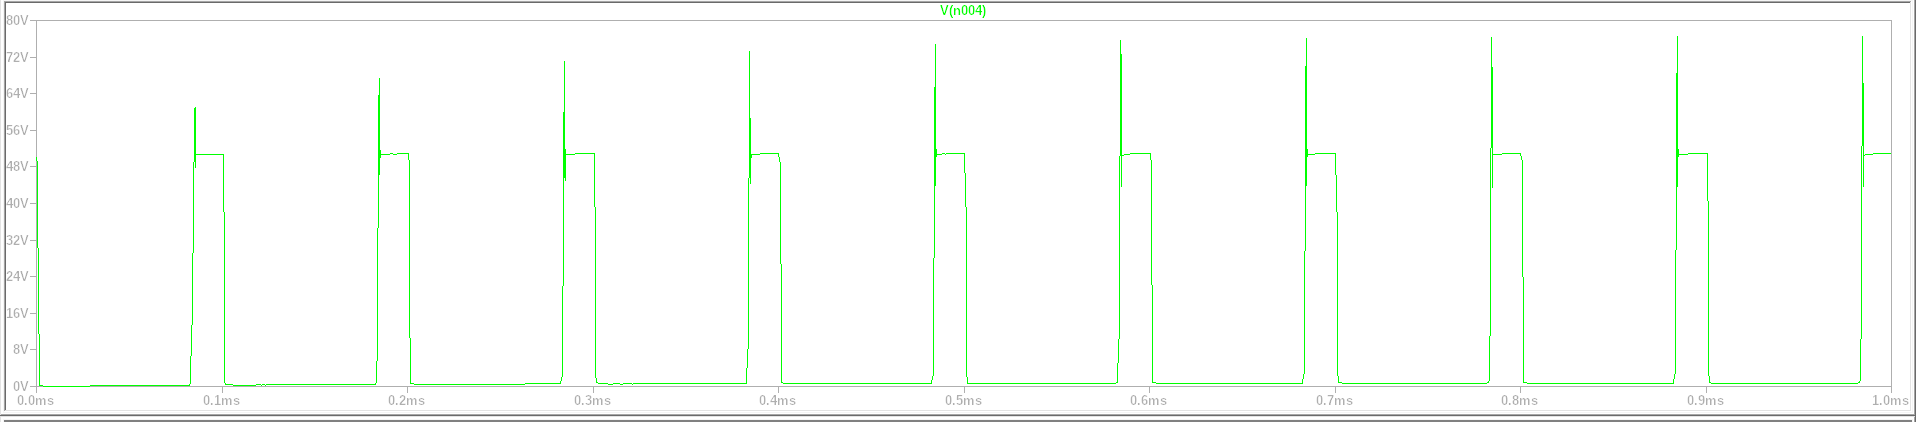
\includegraphics[width=0.8\textwidth]{aun1_rld_with_snubber_rgate100ohm.png}
\caption{Przebieg napiecia na wyjsciu tranzystora MOSFET sterujacego ukladem RLD z rezystancja bramki 100 [\Omega] i z tlumikiem oscylacji D-S}
\end{figure}

\begin{figure}[H]
\centering
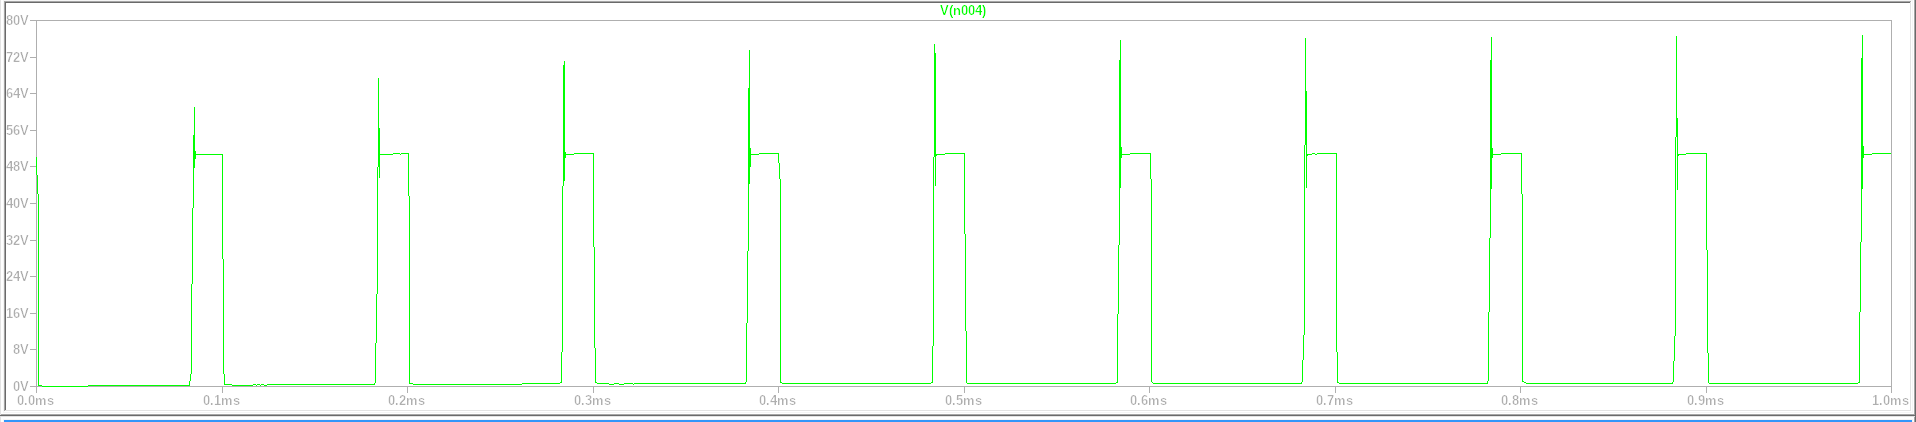
\includegraphics[width=0.8\textwidth]{aun1_rld_with_snubber_rgate10ohm.png}
\caption{Przebieg napiecia na wyjsciu tranzystora MOSFET sterujacego ukladem RLD z rezystancja bramki 10 [\Omega] i z tlumikiem oscylacji D-S}
\end{figure}

\begin{table}[H]
\centering
\begin{tabular}{|l|c|c|}
\hline
\textbf{Tlumik} & \(\mathbf{T_{osc} \ [\mu s]}\) & \(\mathbf{A_{osc} \ [V]}\) \\
\hline
Bez tlumika, \(R_{gate} = 100\,\Omega\) & 1.0958 & 30.7943 \\
\hline
Bez tlumika, \(R_{gate} = 10\,\Omega\) & 1.8058 & 50.8134 \\
\hline
Tlumik, \(R_{gate} = 10\,\Omega\) & 1.0968 & 10.0267 \\
\hline
Tlumik, \(R_{gate} = 100\,\Omega\) & 1.1505 & 10.4941 \\
\hline
\end{tabular}
\caption{Porownanie napiecia na drenie tranzystora MOSFET sterujacym ukladem RLD z oraz bez uzycia tlumika}
\label{tab:oscillation_data}
\end{table}

\end{figure}

\section{Część II}

\subsection{TYPOWA REALIZACJA TORU STEROWANIA TRANZYSTORA MOSFET}

f) Badanie wplywu wartosci komponentow na strate mocy na tranzystorze. Porownanie dynamiki transoptora analogowego i cyfrowego z uwzglednieniem pradu diody. Zaleznosc wytracanej mocy na tranzystorze w zaleznosci od czestotliwosci PWM.

Zapoznano się ze strukturą i zamodelowano typowy tor sterowania tranzystorem MOSFET.
Układ składa się z bloku separacji galwanicznej – transoptora, układu wzmocnienia sygnału oraz gate drivera.
Transoptor zapewnia, że sygnał sterujący jest przekazywany bez elektrycznego połączenia, umożliwiając pracę w układzie o różnych punktach odniesienia masy i chroniąc elektronikę sterującą przed uszkodzeniem.
Gate driver odpowiada za szybkie i pewne przełączanie tranzystora poprzez odpowiednie ładowanie i rozładowywanie jego pojemności bramki, co ma istotny wpływ na straty przełączania oraz niezawodność pracy całego układu.
Do wejścia układu sterującego podawany jest sygnał PWM (ang. Pulse Width Modulation), który steruje pracą transoptora, a w konsekwencji – tranzystora MOSFET. Sygnał ten determinuje częstotliwość oraz czas włączenia tranzystora, wpływając bezpośrednio na charakterystykę napięcia i prądu w obwodzie wyjściowym.\\

Porównano dwa transoptory - analogowy (PC817) oraz cyfrowy (ISOM8710). 
Dodatkowo zbadano wpływ prądu diody na ich dynamikę i przedstawiono na wykresach.\\

\begin{figure}[H]
\centering
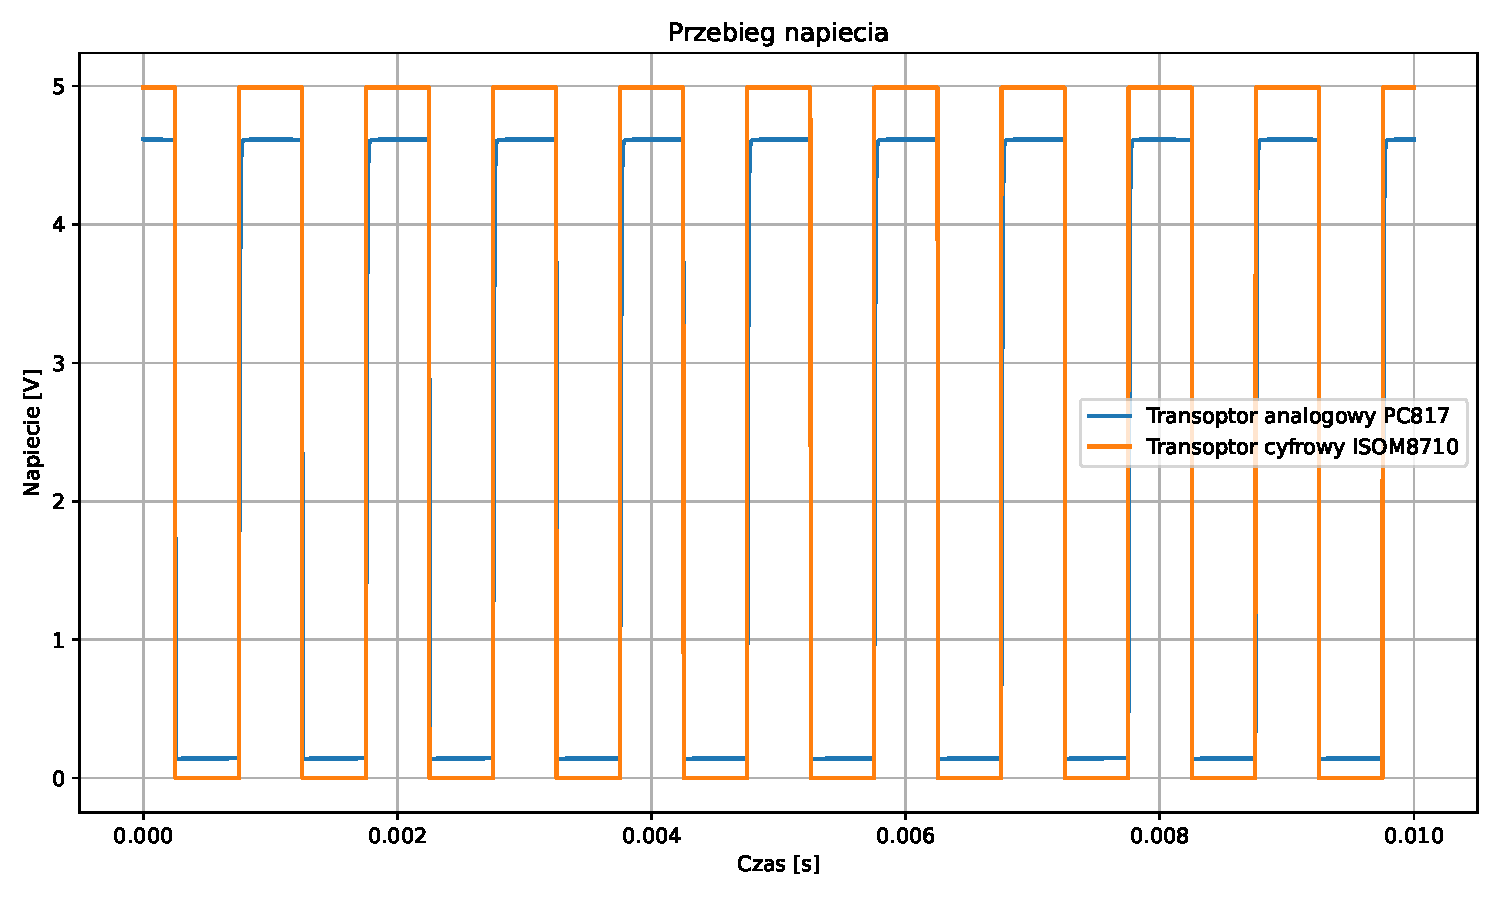
\includegraphics[width=0.8\textwidth]{aun1_gate_circuit_digital_vs_analog_rin100ohm.pdf}
\caption{Przebiegi napiecia na wyjsciu tranzystora MOSFET z transoptorem dla rezystancji wejsciowej 100 [\Omega]}
\end{figure}

\begin{figure}[H]
\centering
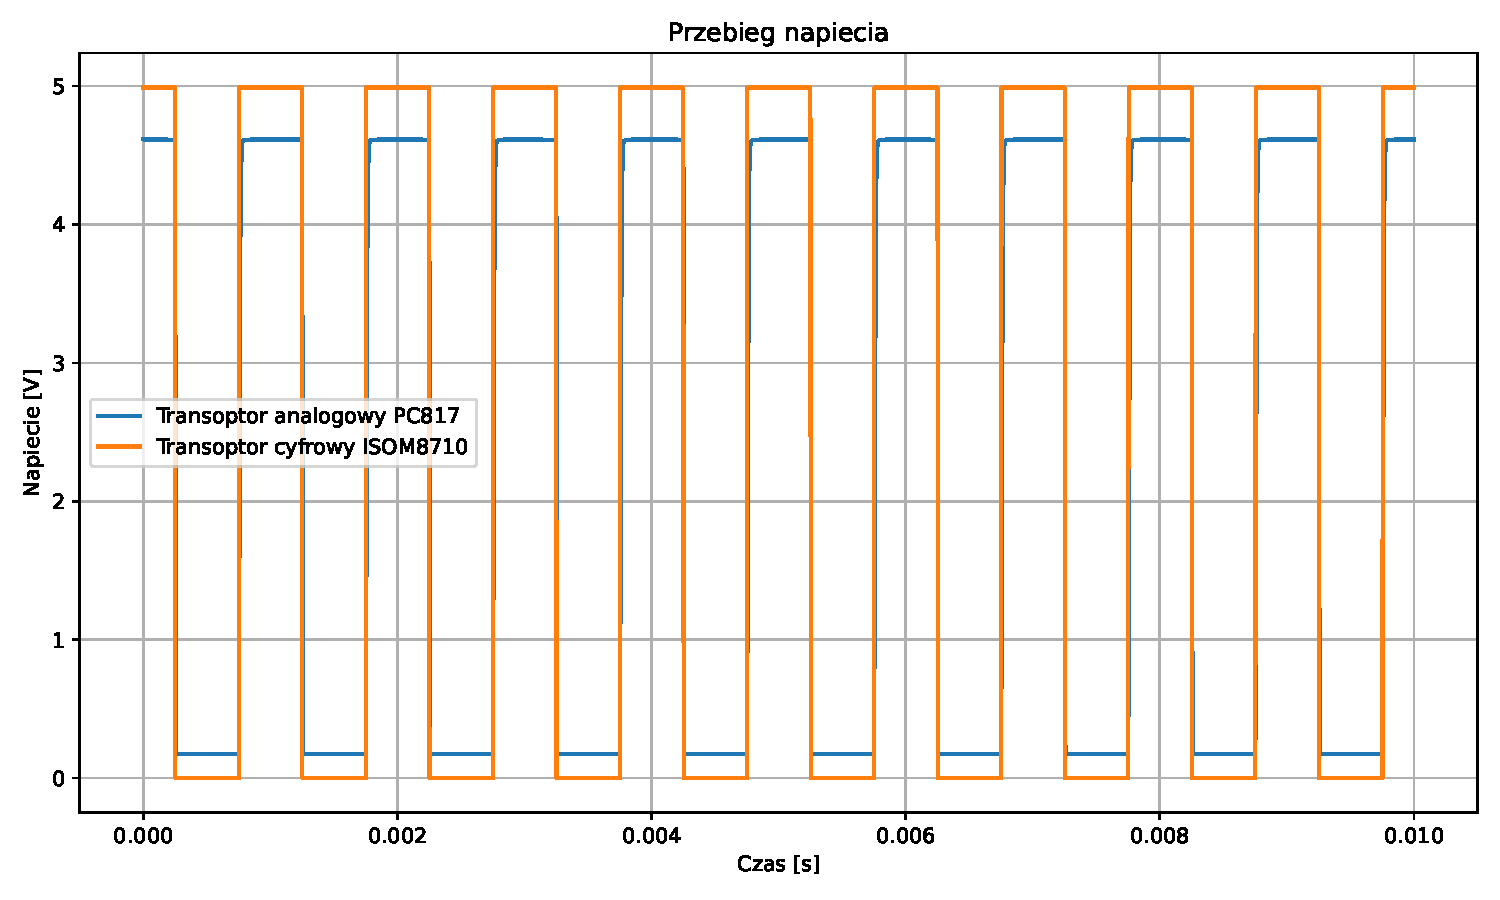
\includegraphics[width=0.8\textwidth]{aun1_gate_circuit_digital_vs_analog_rin230ohm.pdf}
\caption{Przebiegi napiecia na wyjsciu tranzystora MOSFET z transoptorem dla rezystancji wejsciowej 230 [\Omega]}
\end{figure}

\begin{figure}[H]
\centering
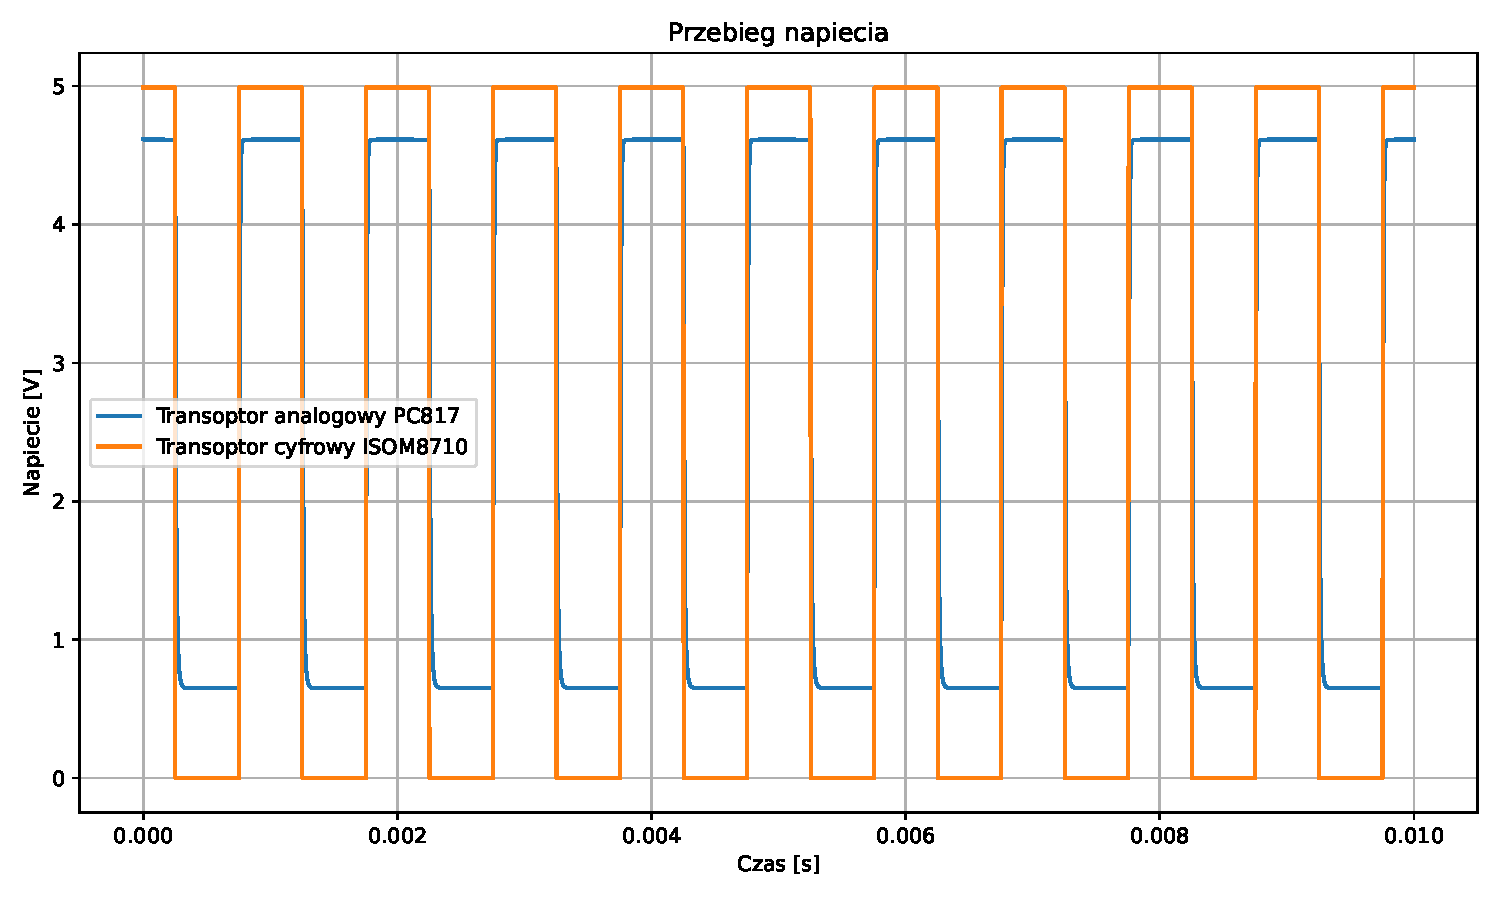
\includegraphics[width=0.8\textwidth]{aun1_gate_circuit_digital_vs_analog_rin500ohm.pdf}
\caption{Przebiegi napiecia na wyjsciu tranzystora MOSFET z transoptorem dla rezystancji wejsciowej 500 [\Omega]}
\end{figure}

\begin{figure}[H]
\centering
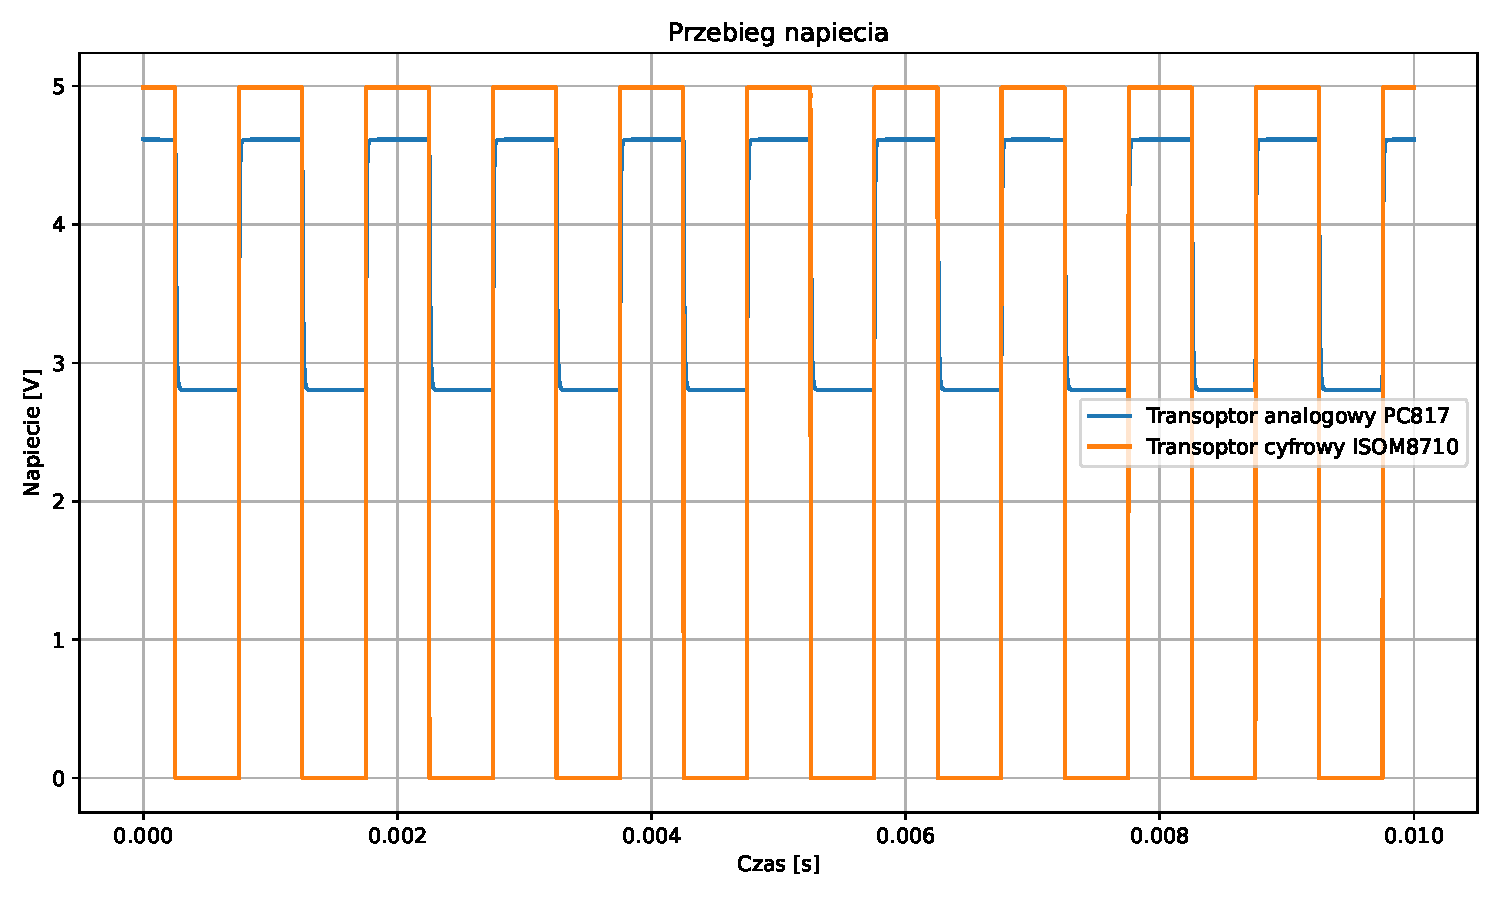
\includegraphics[width=0.8\textwidth]{aun1_gate_circuit_digital_vs_analog_rin1000ohm.pdf}
\caption{Przebiegi napiecia na wyjsciu tranzystora MOSFET z transoptorem dla rezystancji wejsciowej 1000 [\Omega]}
\end{figure}

\begin{table}[H]
\centering
\begin{tabular}{|l|c|c|}
\hline
\textbf{Rezystancja wejściowa} & \(\mathbf{I_{analog} \ [mA]}\) & \(\mathbf{I_{cyfrowy} \ [mA]}\) \\
\hline
100\,$\Omega$ & 18.0 & 14.0 \\
\hline
230\,$\Omega$ & 8.0 & 6.5 \\
\hline
500\,$\Omega$ & 3.8 & 3.2 \\
\hline
1000\,$\Omega$ & 1.9 & 1.6 \\
\hline
1560\,$\Omega$ & 1.3 & 1.0 \\
\hline
\end{tabular}
\caption{Porównanie prądu diody w funkcji rezystancji wejściowej dla sygnału analogowego i cyfrowego}
\label{tab:diode_current_comparison}
\end{table}

Z wykresów widać, że im mniejszy prąd na diodzie tym mniejsza minimalna wartość napięcia na transoptorze analogowym. Natomiast na transoptorze cyfrowym napięcie minimalne się nie zmienia, aż do momentu przekroczenia 1560 \Omega na rezystorze wejściowym - wtedy napięcie ma wartość niezmienną 5V. \\

Dynamika zmienia się także przy zmianie częstotliwości, co pokazano na wykresach: \\

\begin{figure}[H]
\centering
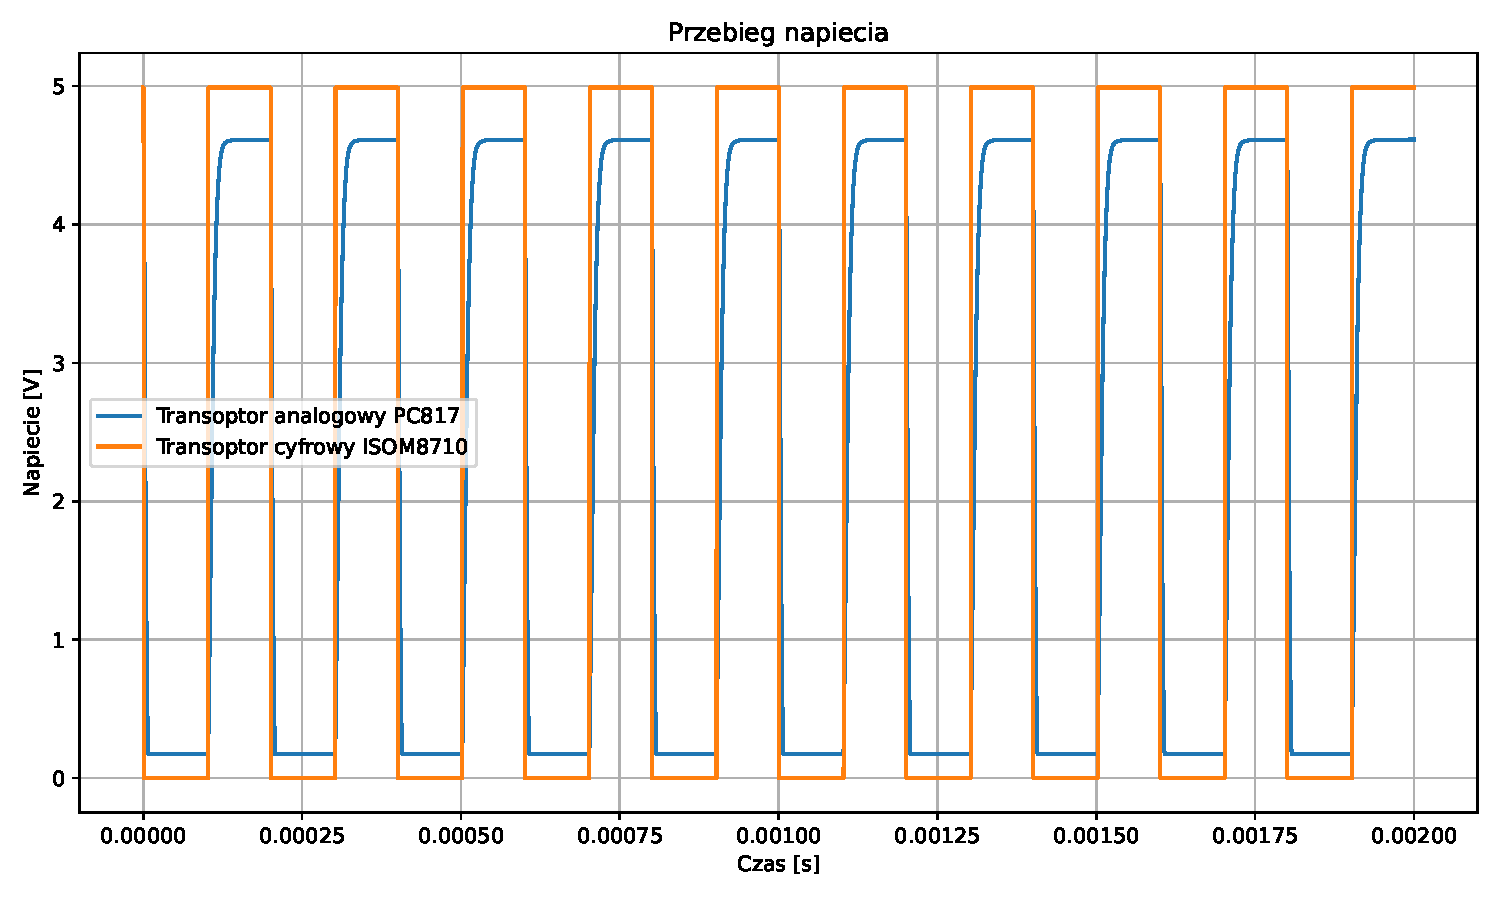
\includegraphics[width=0.8\textwidth]{aun1_gate_circuit_digital_vs_analog_5khz.pdf}
\caption{Przebiegi napiecia na wyjsciu tranzystora MOSFET z transoptorem dla sygnalu PWM o czestotliwosci 5kHz}
\end{figure}

\begin{figure}[H]
\centering
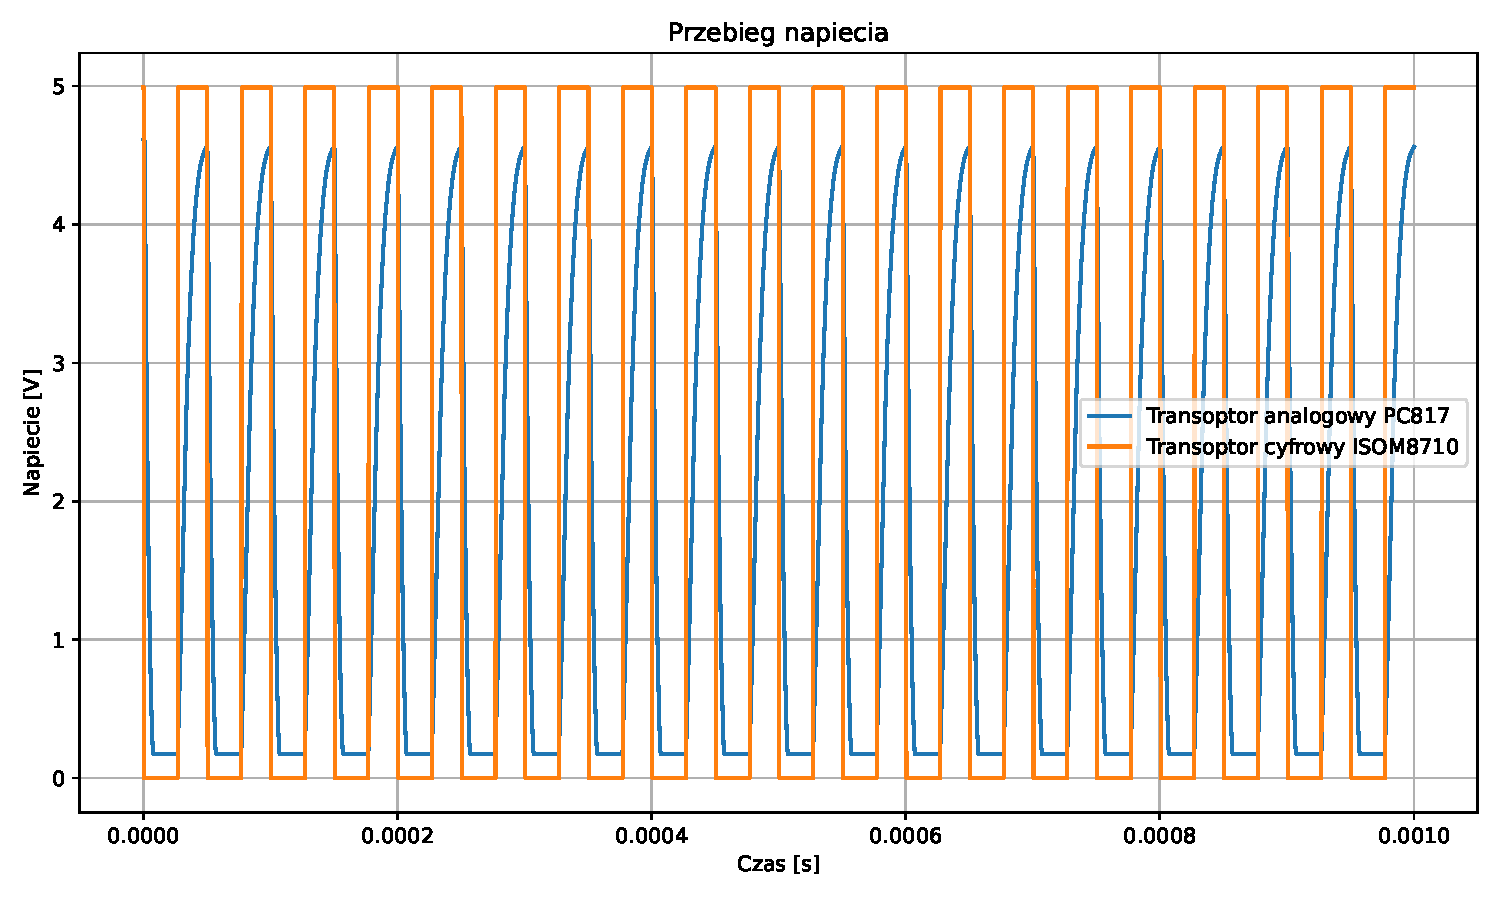
\includegraphics[width=0.8\textwidth]{aun1_gate_circuit_digital_vs_analog_20khz.pdf}
\caption{Przebiegi napiecia na wyjsciu tranzystora MOSFET z transoptorem dla sygnalu PWM o czestotliwosci 20kHz}
\end{figure}

Na wykresach widać, że transoptor analogowy nie radzi sobie tak dobrze jak transoptor cyfrowy dla wysokich częstotliwości.\\

Zbadano średnią moc tranzystorów MOSFET IPW654041CFD7 (MOSFET) i IKQB120N75CP2 (IGBT). \\

\begin{table}[H]
\centering
\resizebox{\textwidth}{!}{%
\begin{tabular}{|l|c|c|}
\hline
\textbf{Częstotliwość [kHz]} & \textbf{Moc wytracana IPW65R041CFD7 (W)} & \textbf{Moc wytracana IKQB120N75CP2 (W)} \\
\hline
1 & 3.5 & 6.6 \\
\hline
5 & 2.2 & 6.4 \\
\hline
10 & 2.5 & 8.33 \\
\hline
25 & 3.8 & 14.8 \\
\hline
50 & 6.1 & 26.8 \\
\hline
100 & 12.1 & 52.3 \\
\hline
\end{tabular}%
}
\caption{Średnia moc wytracana na tranzystorze w zależności od częstotliwości}
\end{table}

Widać, że im większa częstotliwość tym większe straty na tranzystorach. Patrząc na straty mocy to lepiej radzi sobie tranzystor IPW654041CFD7, niż IKQB120N75CP2.\\

\subsection{MOSTKOWE UKŁADY WZMACZNIACZY TRANZYSTOROWYCH}

g) Problemy mostkow mocy

Mostek mocy to układ elektroniczny wykorzystywany do sterowania przepływem prądu przez obciążenie, najczęściej silnik. Najpopularniejszą konfiguracją jest tzw. mostek H, który składa się z czterech tranzystorów mocy. Dzięki odpowiedniemu przełączaniu tych tranzystorów możliwe jest sterowanie kierunkiem oraz wartością prądu płynącego przez obciążenie. Mostki mocy znajdują zastosowanie w układach napędowych i przekształtnikach, a ich działanie opiera się na szybkim przełączaniu elementów półprzewodnikowych w celu efektywnego zarządzania energią.\\

W mostku H kluczowe są trzy rodzaje sterowania:
\begin{itemize}
\item unipolarny,
\item quasi-bipolarny,
\item bipolarny.
\end{itemize}
\vspace{1em}

h) Analiza dzialania ukladu sterowania bipolarnego, unipolarnego, quasi-bipolarnego

W układach z obciążeniem RLE (rezystancja, indukcyjność i źródło siły elektromotorycznej), istotnym zjawiskiem jest konieczność zapewnienia ścieżki demagnetyzacji dla prądu cewki. Podczas wyłączania tranzystorów sterujących, energia zgromadzona w indukcyjności nie może zostać natychmiast rozproszona. W takim przypadku pojawiają się przepięcia i zakłócenia, o ile nie zostanie zapewniona odpowiednia ścieżka dla tego prądu.\\

\textbf{Sterowanie unipolarne:}
W tym trybie tranzystory włączane są na przemian tylko w jednej gałęzi mostka (np. górnej). Prąd powrotny z cewki płynie przez diody swobodne w dolnej gałęzi. Ścieżka demagnetyzacji realizowana jest wyłącznie przez te diody, co powoduje wolniejszą dynamikę wyłączania i dłuższy czas ustalania się prądu.
Napięcie wyjściowe przyjmuje wartości +U oraz 0 V, ponieważ prąd jest kierowany tylko przez jedną gałąź mostka, a powrót odbywa się przez diody swobodne.\\

\textbf{Sterowanie quasi-bipolarne:}
Jest to tryb pośredni, gdzie w każdej połowie okresu włączany jest jeden tranzystor, natomiast przeciwny tranzystor w drugiej gałęzi jest wyłączony. Demagnetyzacja cewki odbywa się przez diody swobodne przeciwległej gałęzi, które stanowią naturalną ścieżkę dla prądu indukowanego. Dzięki temu dynamika pracy jest lepsza niż w trybie unipolarnym, a układ zachowuje prostotę sterowania i mniejsze straty energetyczne.
Napięcie może przyjmować wartości +U, –U oraz 0 V, ponieważ każda z połówek cyklu wykorzystuje inną gałąź mostka. Zmiana polaryzacji odbywa się za pośrednictwem diod swobodnych, co umożliwia krótkotrwałe stany zerowe.\\

\textbf{Sterowanie bipolarne:}
Tranzystory włączane są naprzemiennie w obu gałęziach mostka, co pozwala na aktywne sterowanie przepływem prądu w obydwu kierunkach. W momencie przełączania prąd z cewki jest wymuszany przez aktywnie sterowany tranzystor w drugiej gałęzi, co zapewnia najszybszą i najbardziej precyzyjną ścieżkę demagnetyzacji. Odbywa się to jednak kosztem wyższych strat mocy i bardziej skomplikowanego układu sterowania.
Napięcie wyjściowe skacze bezpośrednio między +U a –U. W idealnym przypadku nie występuje 0 V, chyba że w czasie przełączeń PWM (np. dead-time). Umożliwia to najbardziej dynamiczne sterowanie prądem.\\

i) Model bipolarnego i unipolarnego sterowania

Zamodelowano w matlabie i pokazano na wykresach sterowanie bipolarne i unipolarne silnika oraz jak to wpływa na jego prędkość:\\

\begin{figure}[H]
\centering
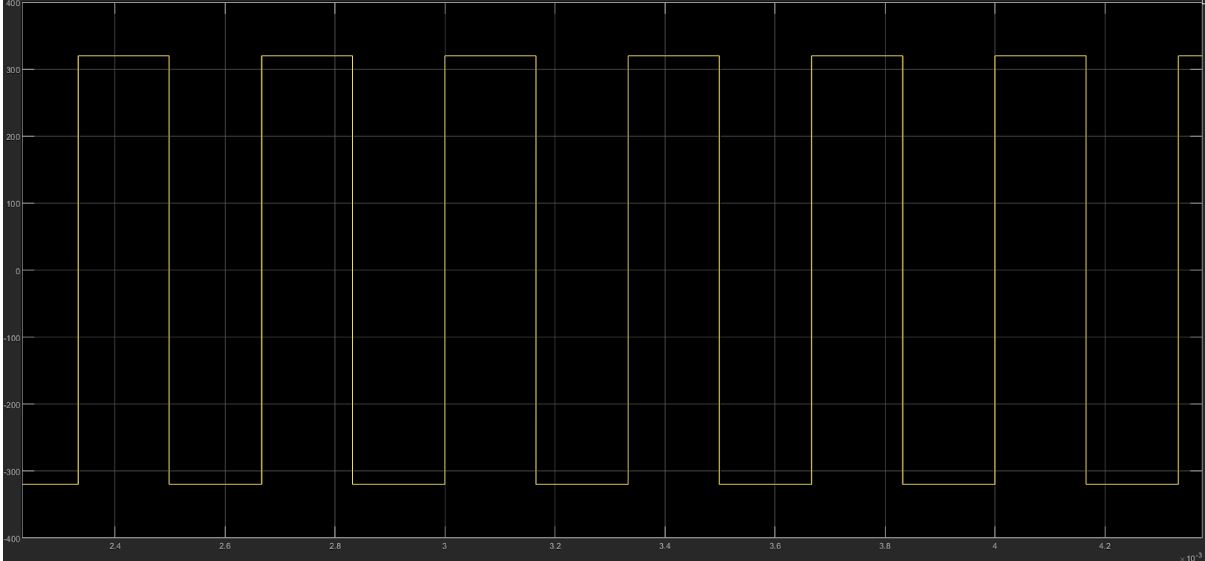
\includegraphics[width=0.8\textwidth]{aun1_bipolar_bridge.png}
\caption{Przebieg napiecia na silniku przy mostku sterowanym bipolarnie}
\end{figure}

\begin{figure}[H]
\centering
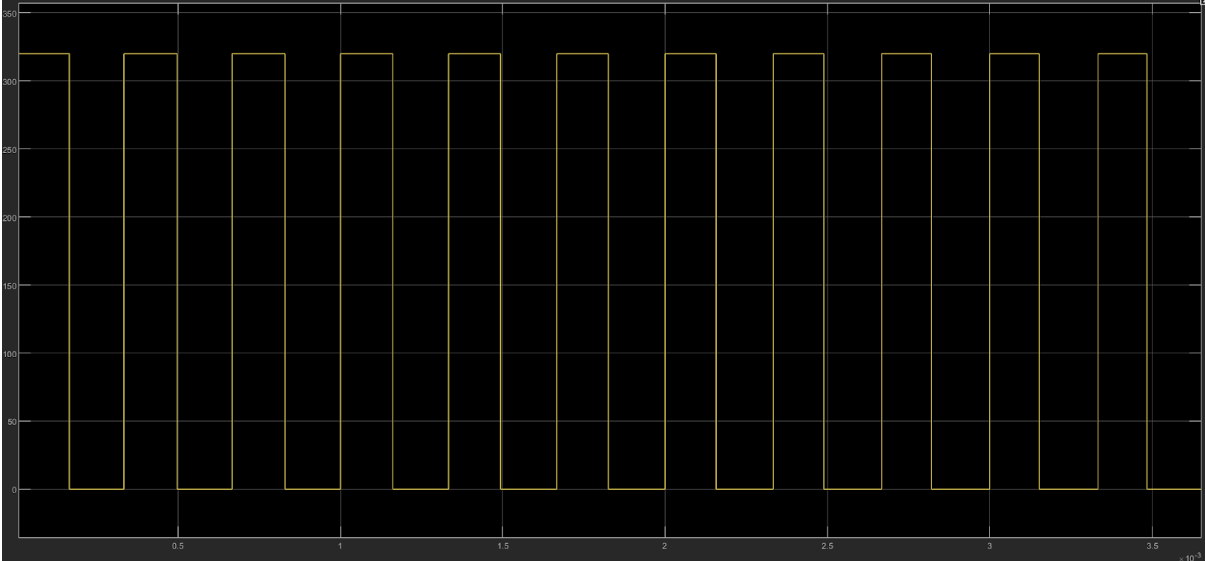
\includegraphics[width=0.8\textwidth]{aun1_unipolar_bridge.png}
\caption{Przebieg napiecia na silniku przy mostku sterowanym unipolarnie}
\end{figure}

\begin{figure}[H]
\centering
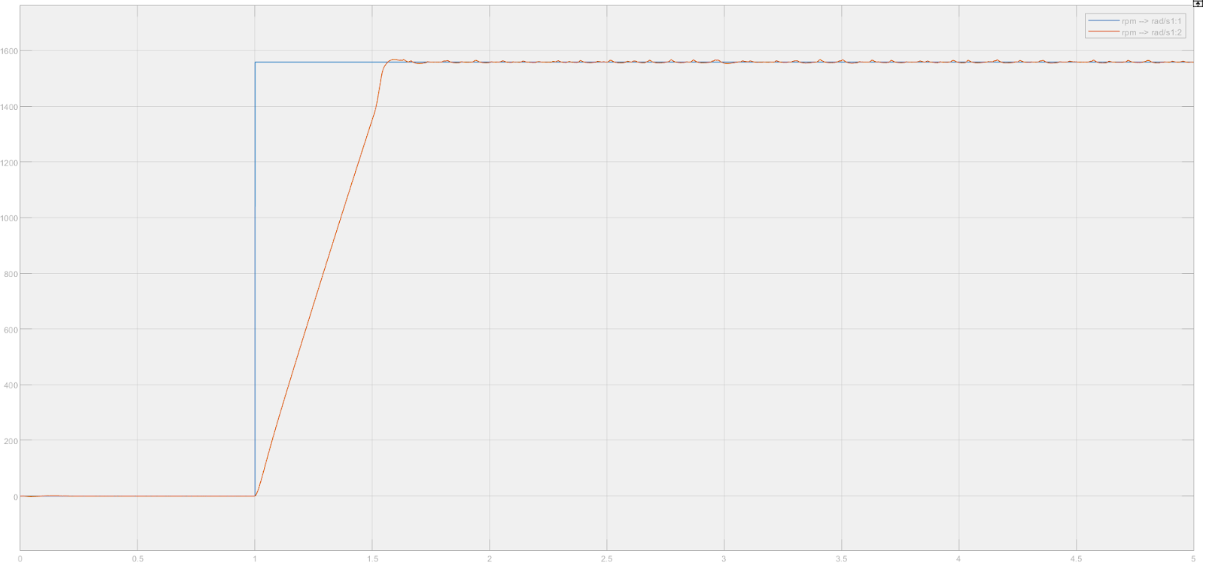
\includegraphics[width=0.8\textwidth]{aun1_bipolar_bridge2.png}
\caption{Przebieg predkosci na silniku przy mostku sterowanym bipolarnie}
\end{figure}

\begin{figure}[H]
\centering
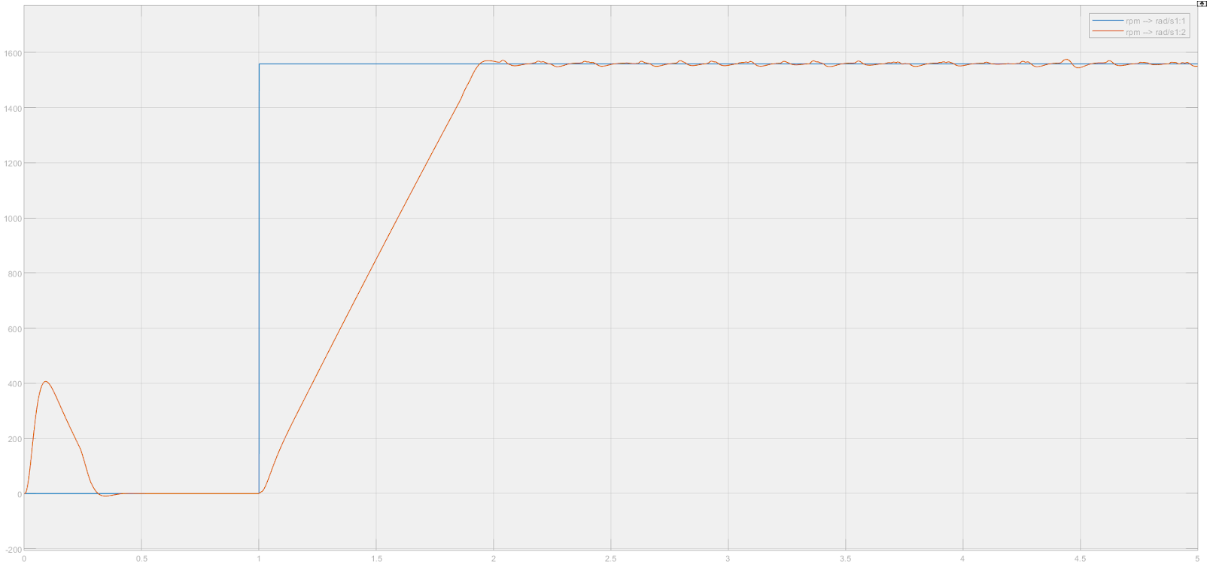
\includegraphics[width=0.8\textwidth]{aun1_unipolar_bridge2.png}
\caption{Przebieg predkosci na silniku przy mostku sterowanym unipolarnie}
\end{figure}

Z wykresów wynika, że przy sterowaniu unipolarnym dynamika układu jest gorsza, a odpowiedź ustala się wolniej. Sterowanie to jest jednak bardziej efektywne energetycznie.\\

\section{Część III}

\subsection{BADANIA EKSPERYMENTALNE}

j) Przebiegi prądów oraz napięć na stanowiskach eksperymentalnych

Uwaga: brak jednostek na osi OY spowodowany jest faktem, ze dane
zapisane byly w formacie raw, niezeskalowane.\\

Regulacja predkosci odbywa sie przez zmiane czestotliwosci pradu i napiecia, amplituda pozostaje stala.\\

Przebiegi napiecia i pradu na stanowisku Alspa.\\

\begin{figure}[H]
\centering
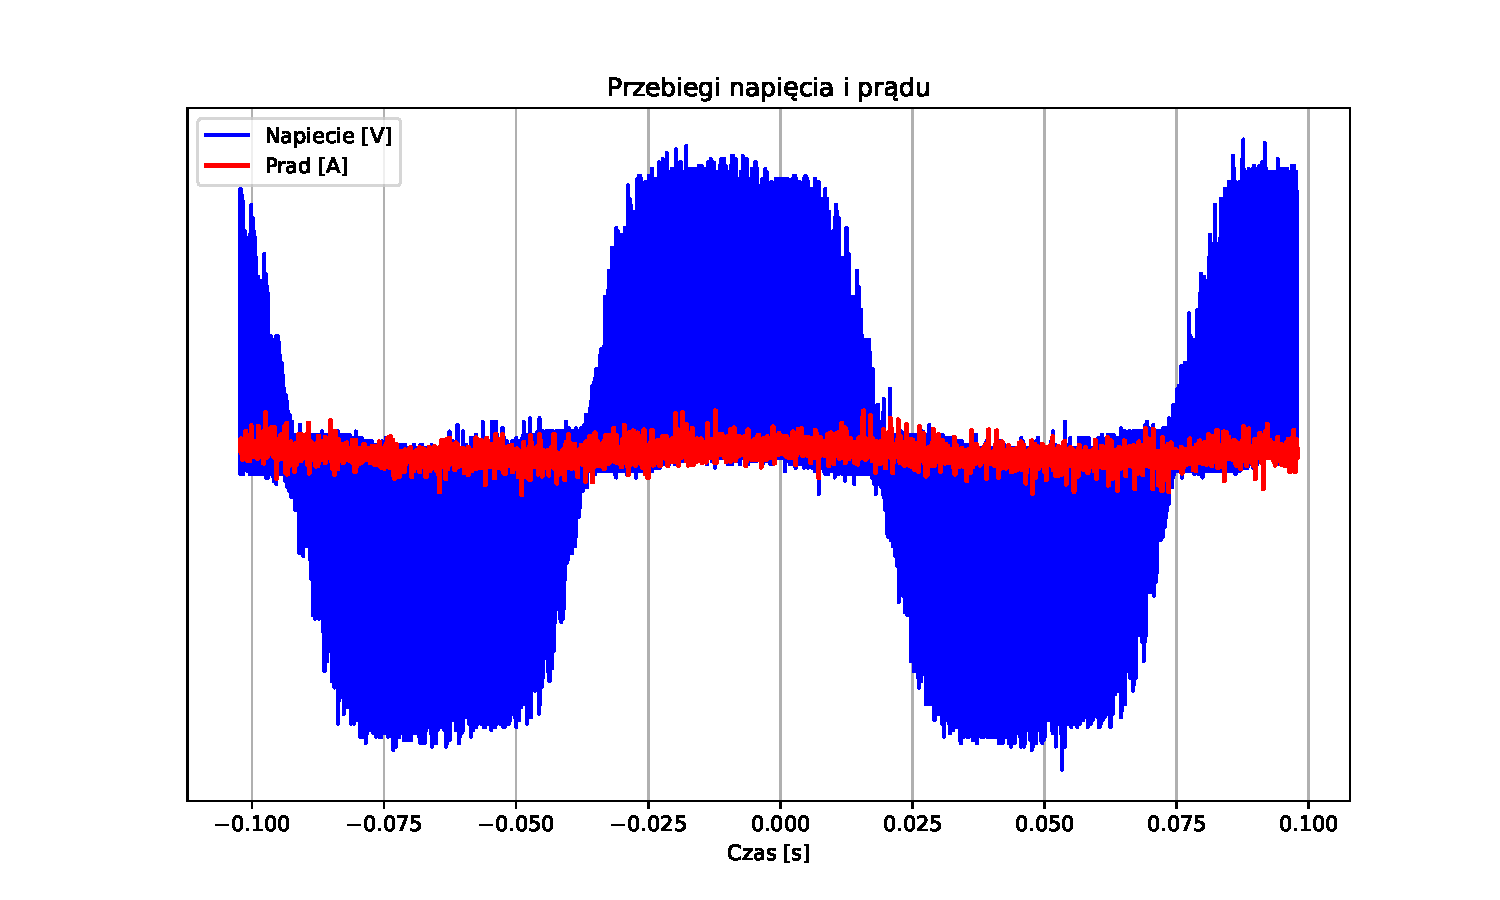
\includegraphics[width=0.8\textwidth]{aun1_alspa_rpm300.pdf}
\caption{Przebieg napiecia oraz pradu na stanowisku Alspa przy predkosci katowej 300 [RPM]}
\end{figure}

\begin{figure}[H]
\centering
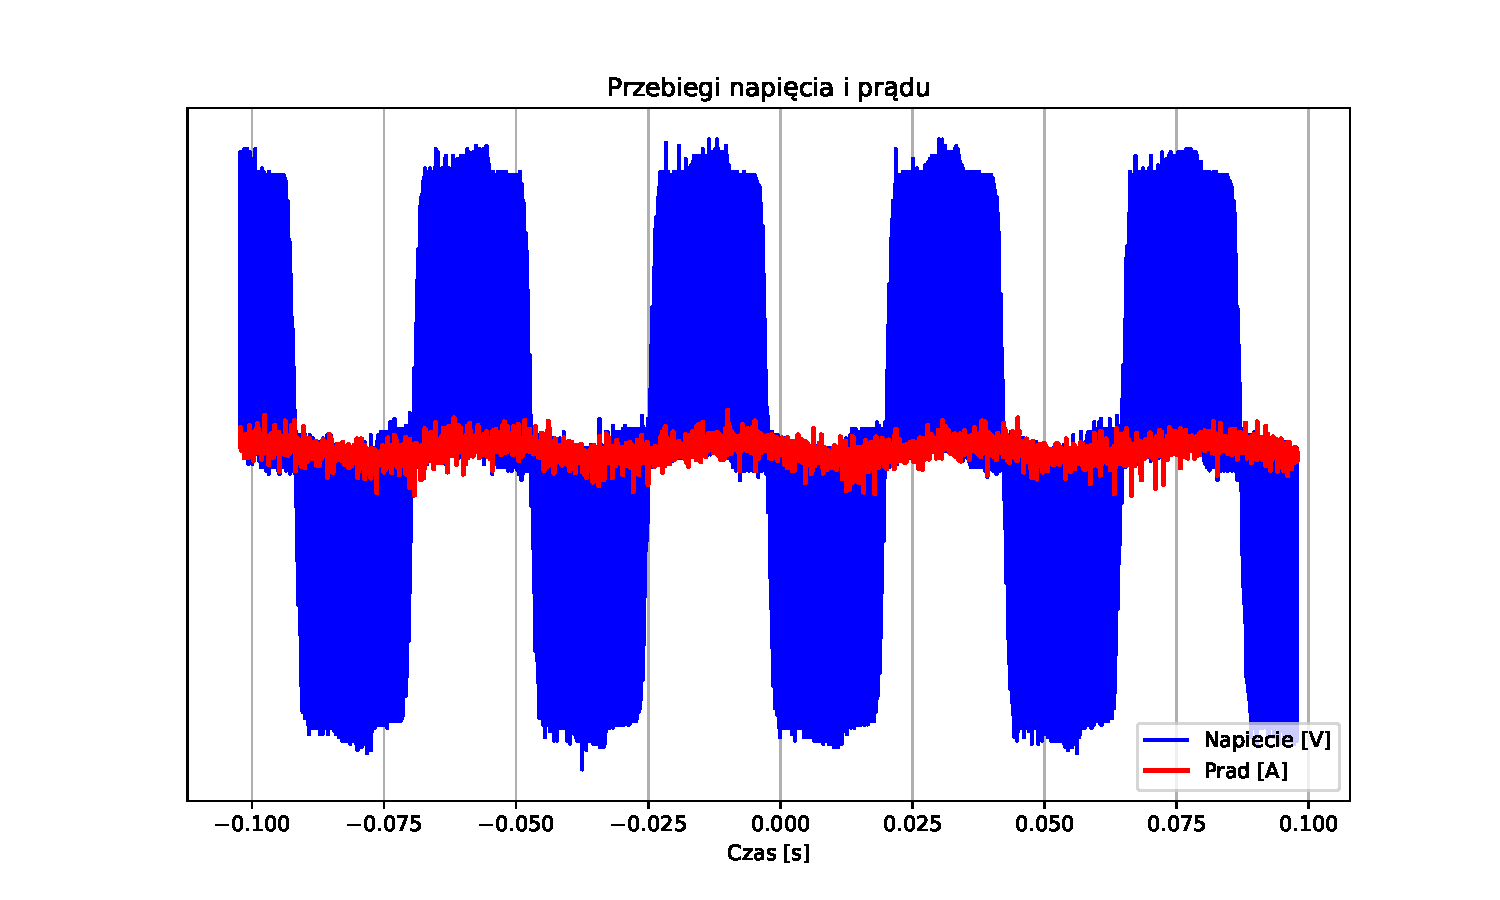
\includegraphics[width=0.8\textwidth]{aun1_alspa_rpm600.pdf}
\caption{Przebieg napiecia oraz pradu na stanowisku Alspa przy predkosci katowej 600 [RPM]}
\end{figure}

\begin{figure}[H]
\centering
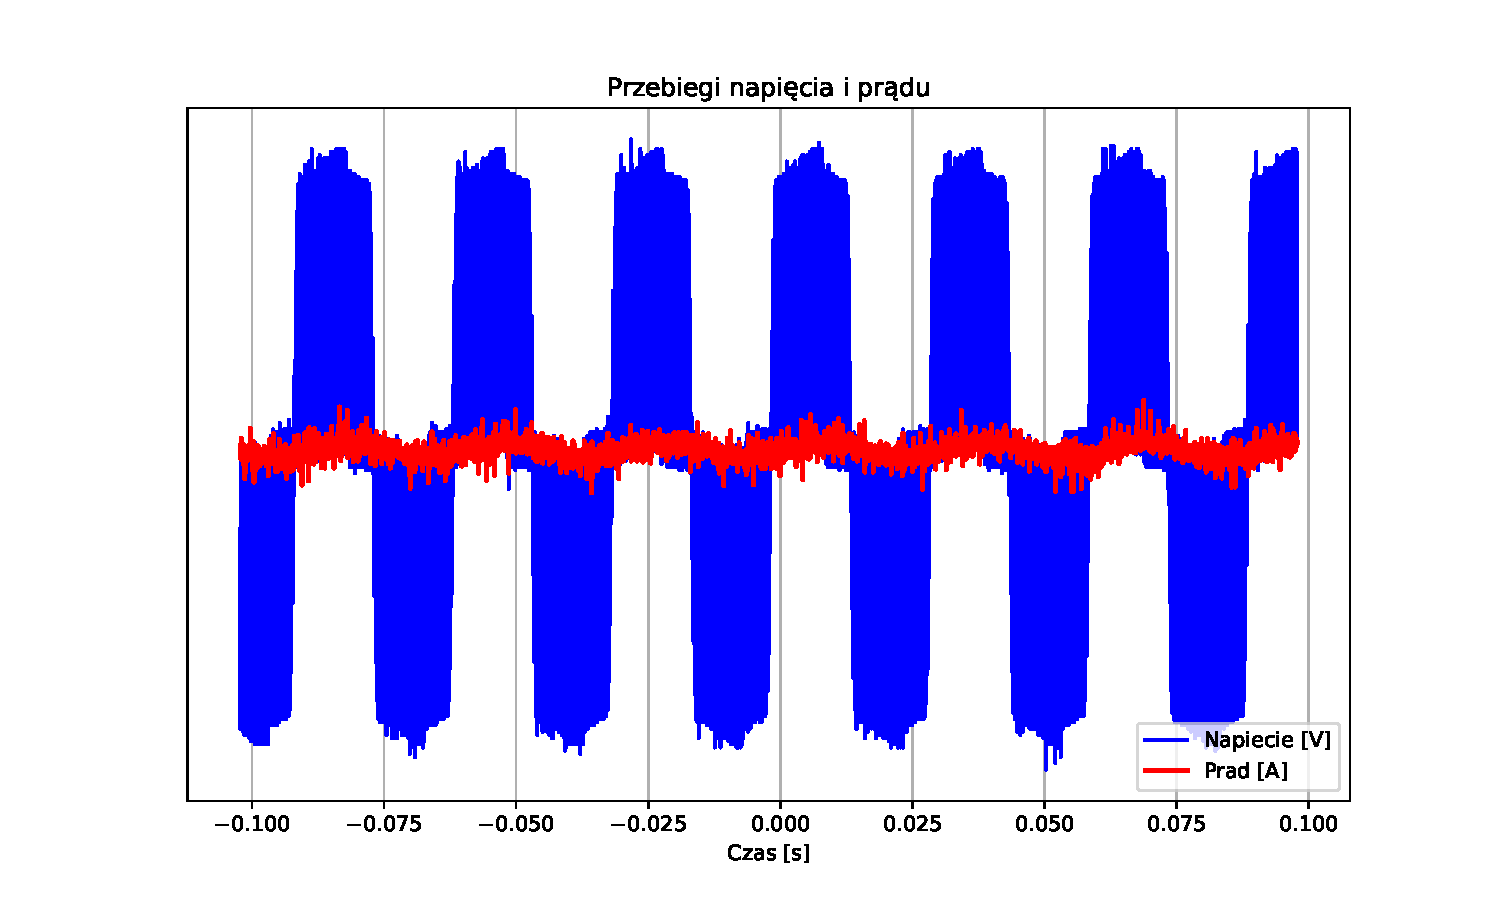
\includegraphics[width=0.8\textwidth]{aun1_alspa_rpm900.pdf}
\caption{Przebieg napiecia oraz pradu na stanowisku Alspa przy predkosci katowej 900 [RPM]}
\end{figure}

Przebiegi napiecia i pradu na stanowisku Microverter.\\

\begin{figure}[H]
\centering
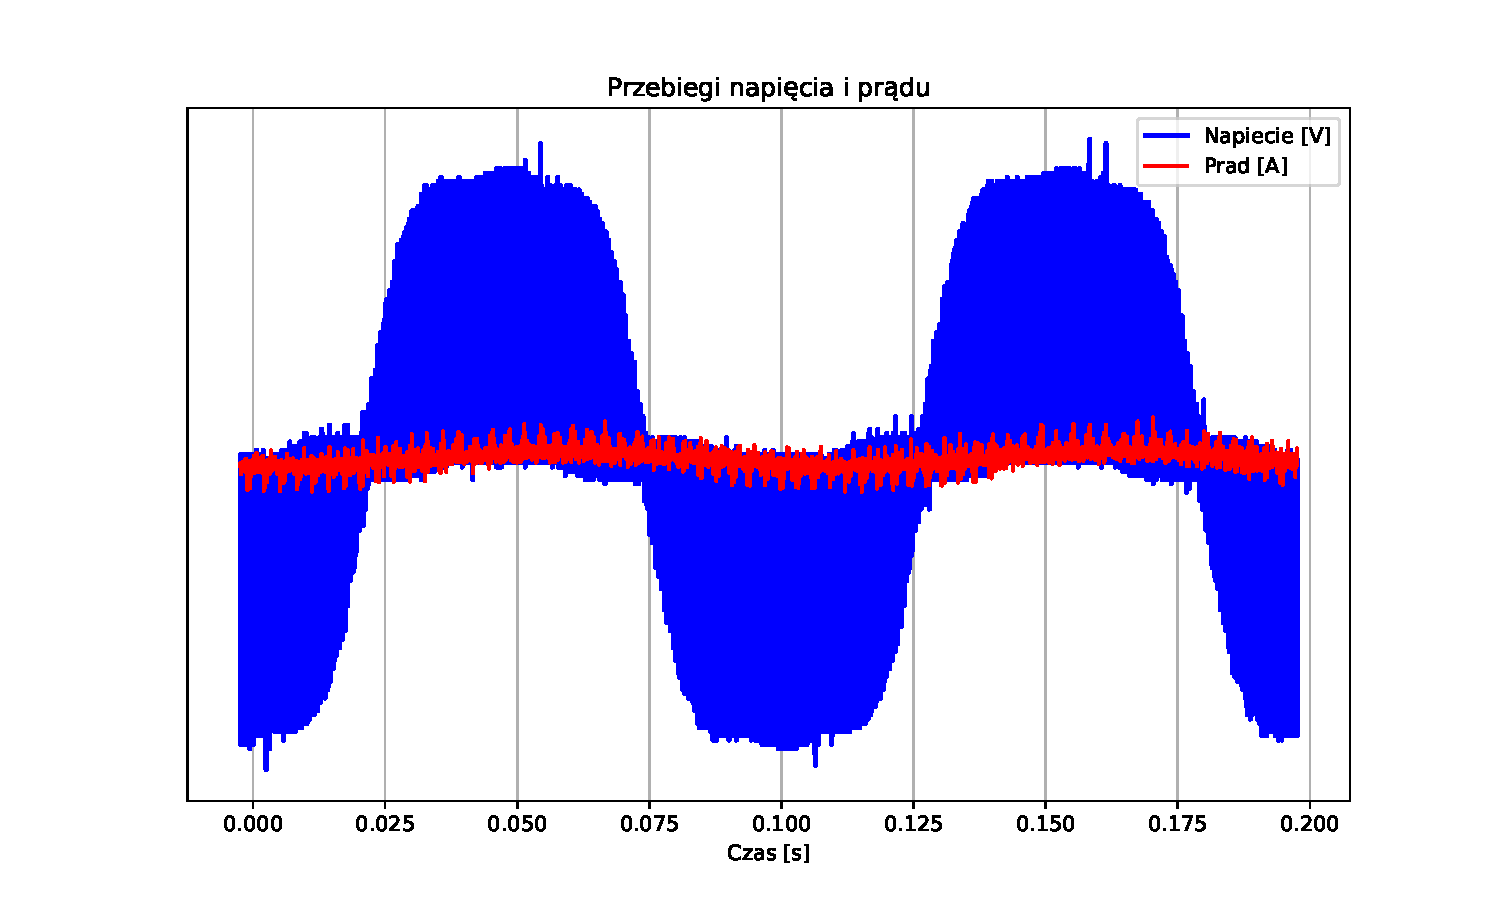
\includegraphics[width=0.8\textwidth]{aun1_microverter_rpm300.pdf}
\caption{Przebieg napiecia oraz pradu na stanowisku Microverter przy predkosci katowej 300 [RPM]}
\end{figure}

\begin{figure}[H]
\centering
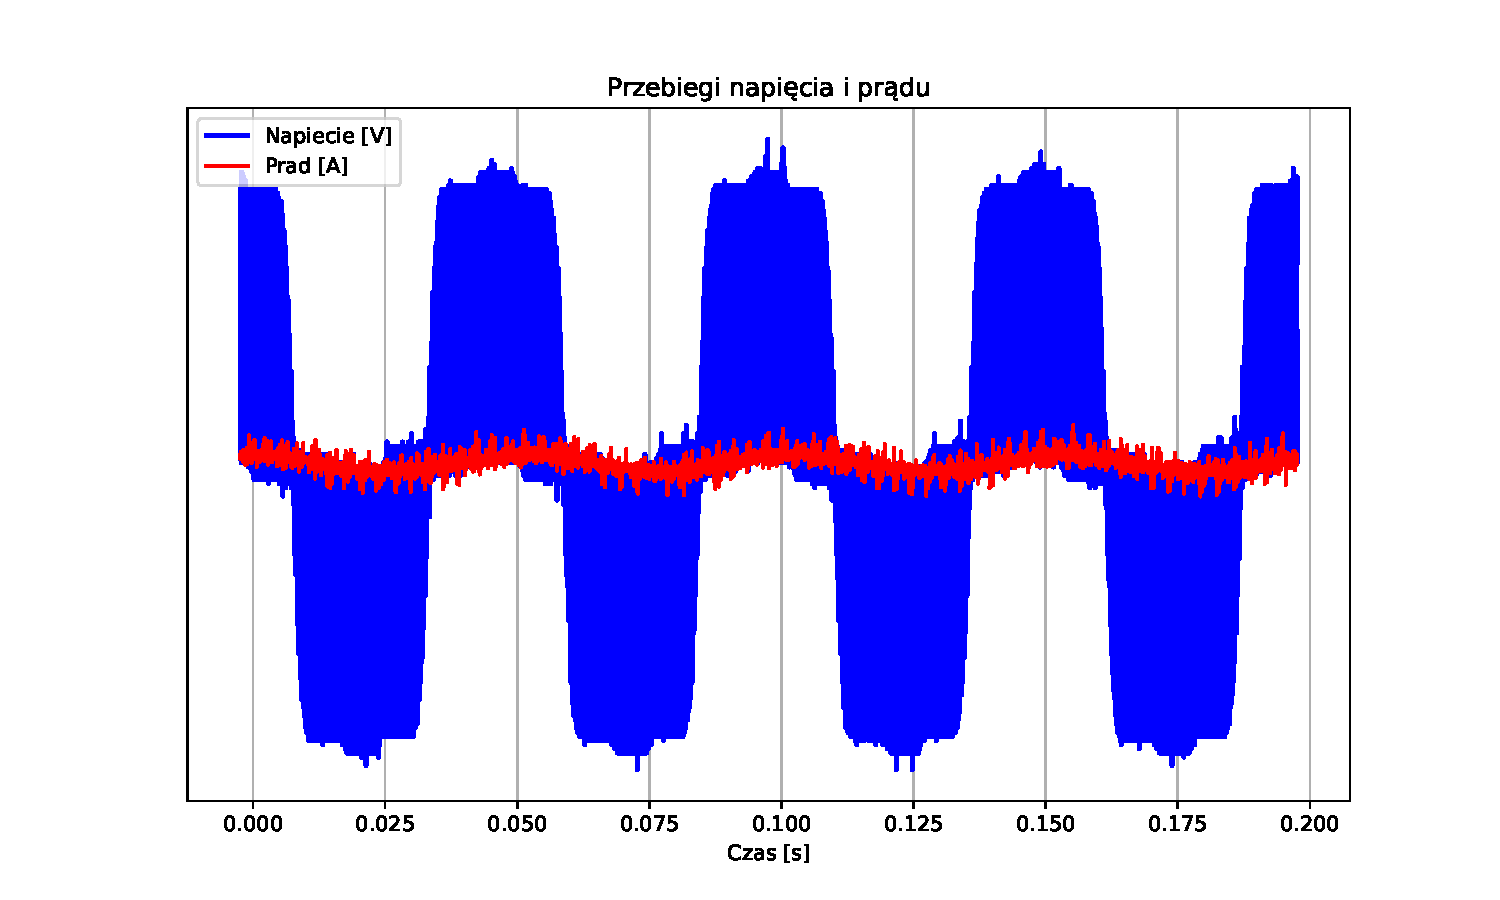
\includegraphics[width=0.8\textwidth]{aun1_microverter_rpm600.pdf}
\caption{Przebieg napiecia oraz pradu na stanowisku Microverter przy predkosci katowej 600 [RPM]}
\end{figure}

\begin{figure}[H]
\centering
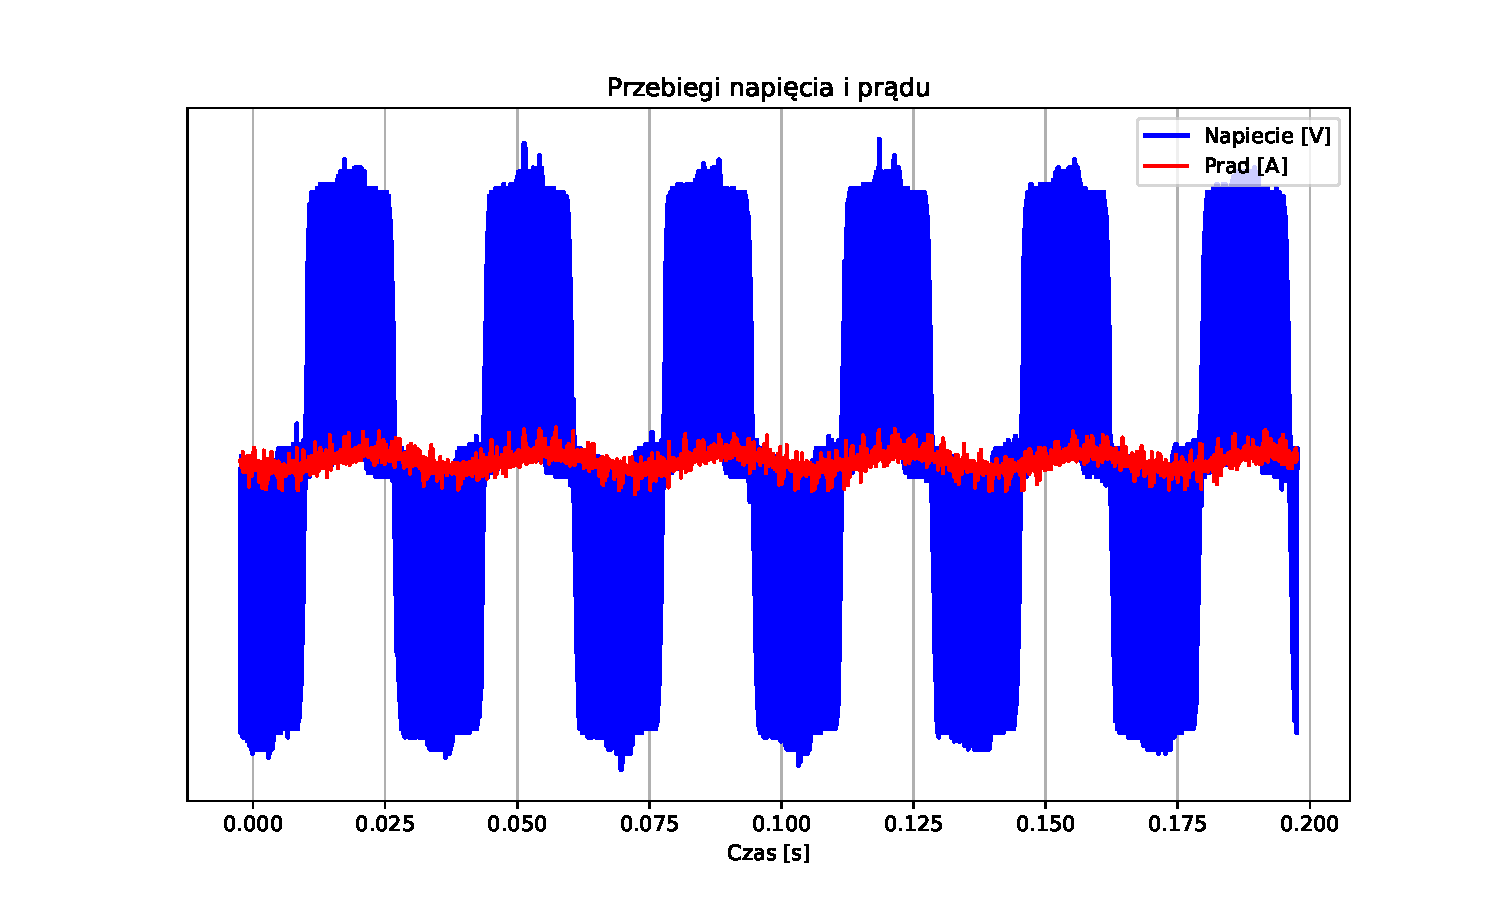
\includegraphics[width=0.8\textwidth]{aun1_microverter_rpm900.pdf}
\caption{Przebieg napiecia oraz pradu na stanowisku Microverter przy predkosci katowej 900 [RPM]}
\end{figure}

Jak widzimy, napęd Unidrive charakteryzuje się mniejsza czestotliwoscia i wieksza amplituda mierzonych wielkosci niz naped Alspa.\\

Przebiegi napiecia i pradu na stanowisku Unidrive.\\

\begin{figure}[H]
\centering
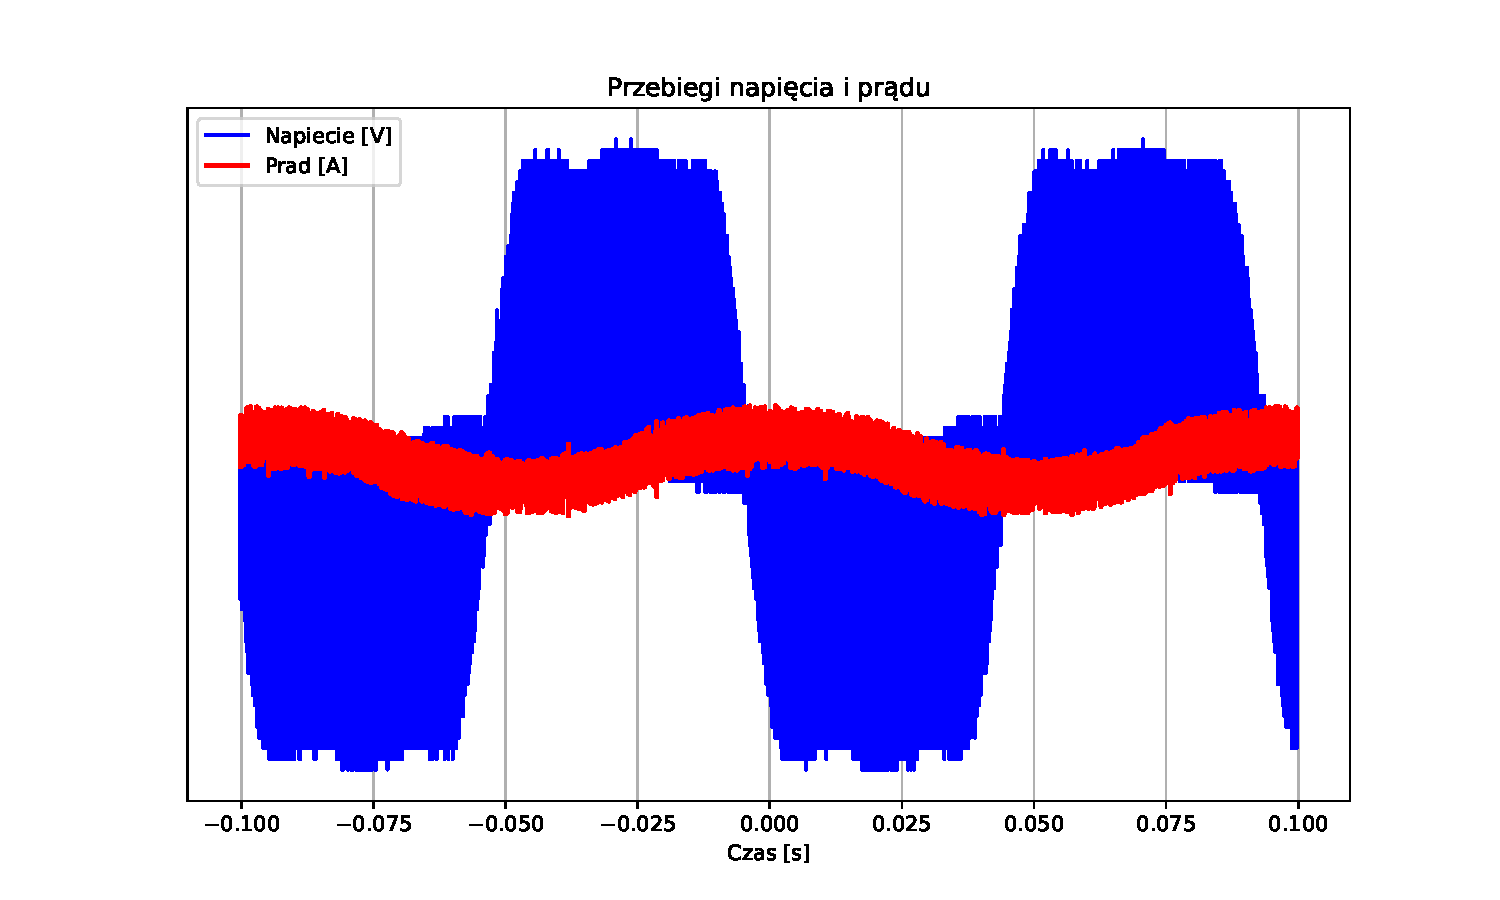
\includegraphics[width=0.8\textwidth]{aun1_unidrive_rpm300.pdf}
\caption{Przebieg napiecia oraz pradu na stanowisku Unidrive przy predkosci katowej 300 [RPM]}
\end{figure}

\begin{figure}[H]
\centering
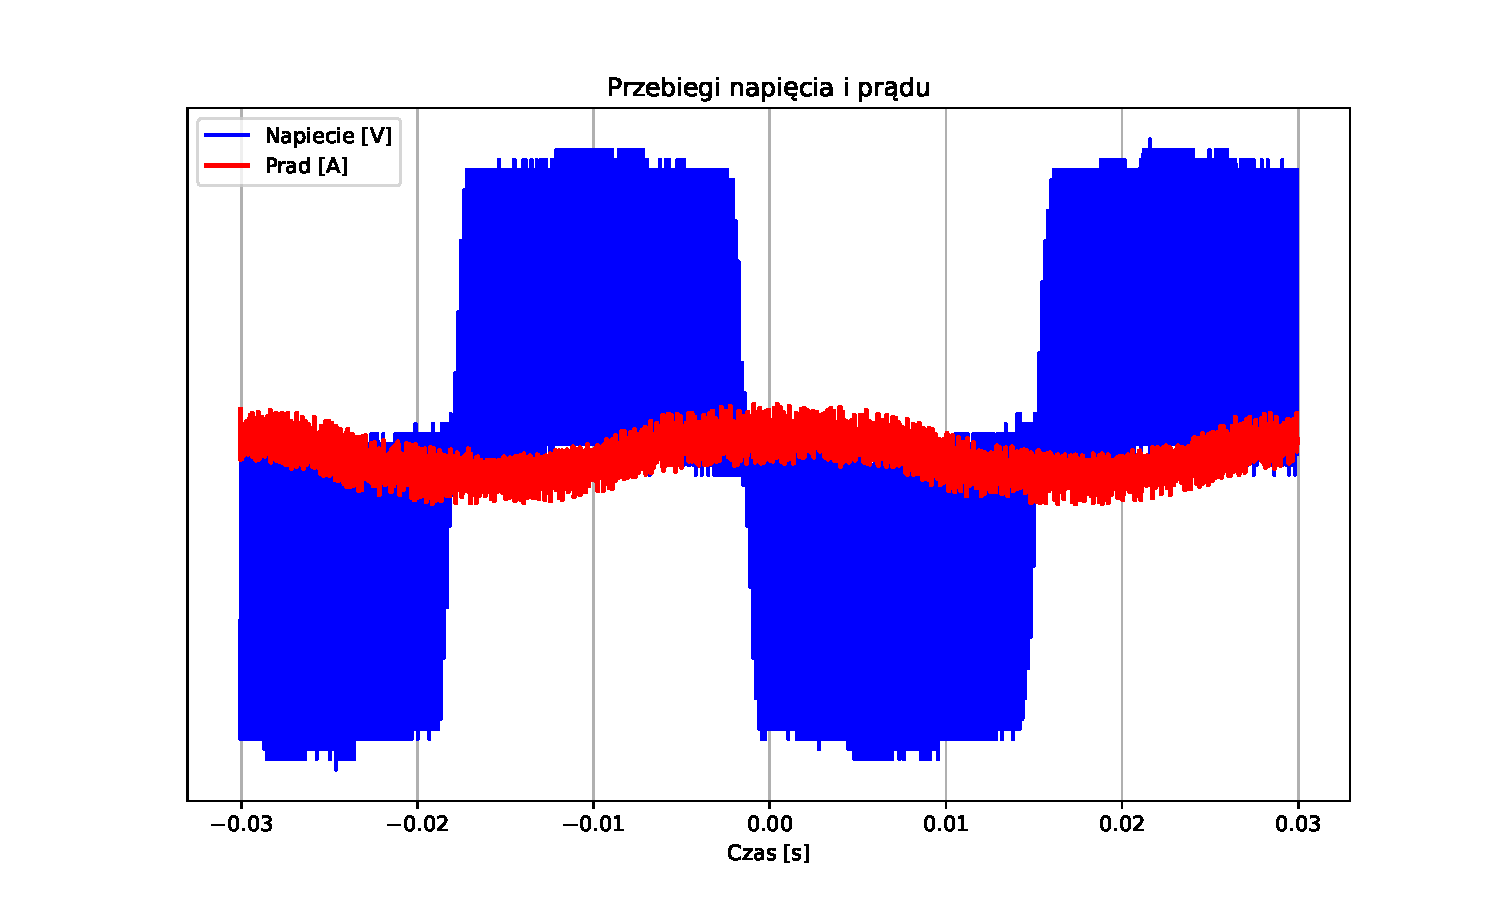
\includegraphics[width=0.8\textwidth]{aun1_unidrive_rpm600.pdf}
\caption{Przebieg napiecia oraz pradu na stanowisku Unidrive przy predkosci katowej 600 [RPM]}
\end{figure}

\begin{figure}[H]
\centering
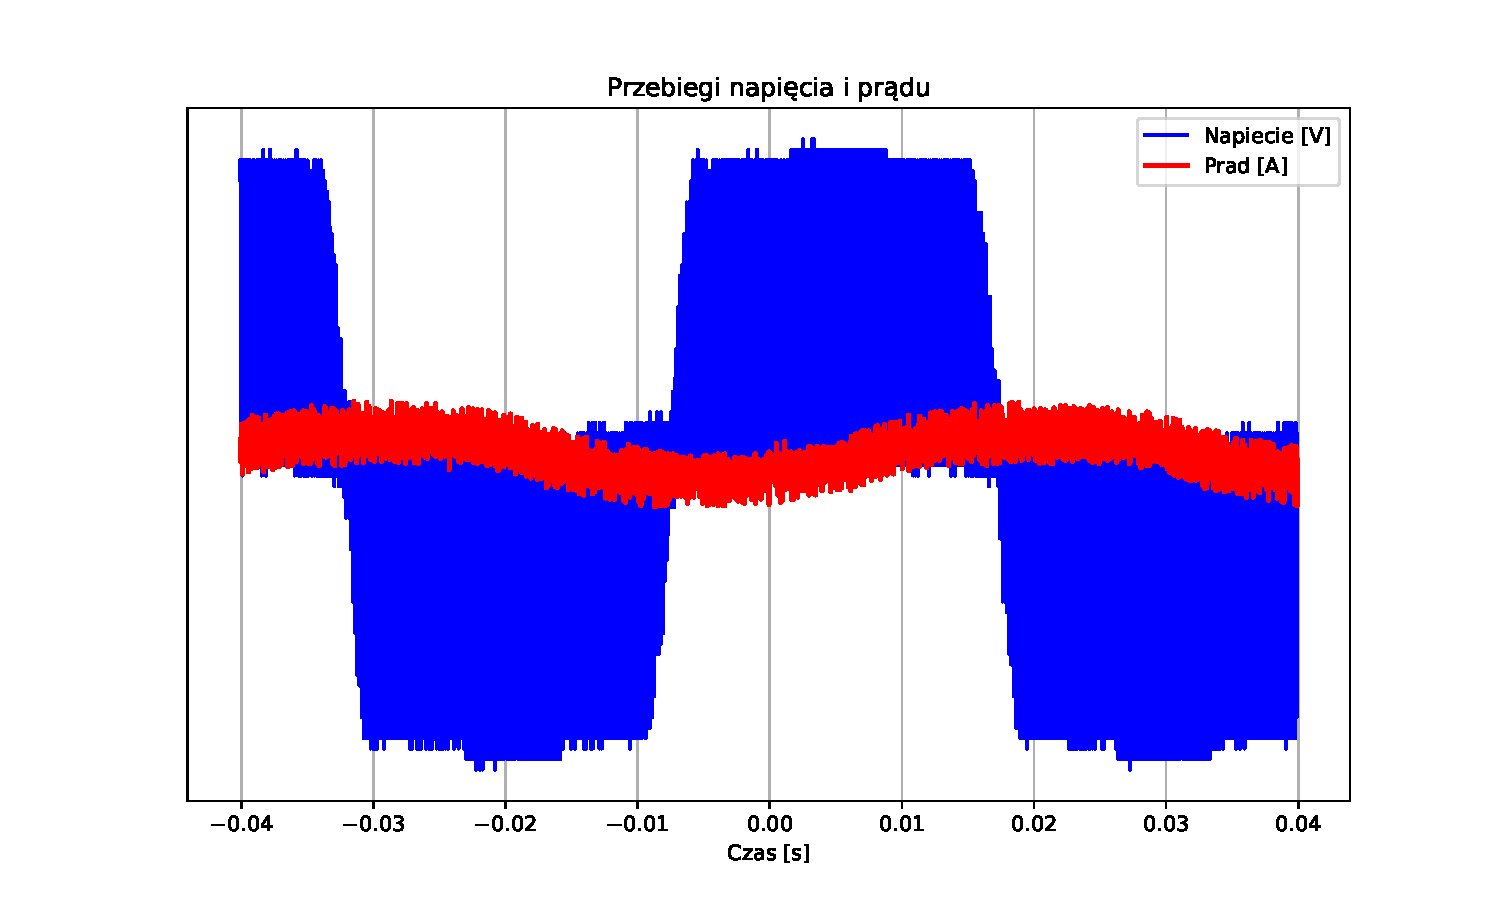
\includegraphics[width=0.8\textwidth]{aun1_unidrive_rpm900.pdf}
\caption{Przebieg napiecia oraz pradu na stanowisku Unidrive przy predkosci katowej 900 [RPM]}
\end{figure}

Jak widzimy, podobnie do napedu Microverter, napęd Unidrive charakteryzuje się mniejsza czestotliwoscia i wieksza amplituda mierzonych wielkosci niz naped Alspa.\\

\section{Część IV}

\subsection{MOSTEK TYRYSTOROWY}

Przebiegi napiecia i pradu na stanowisku DML.\\

\begin{figure}[H]
\centering
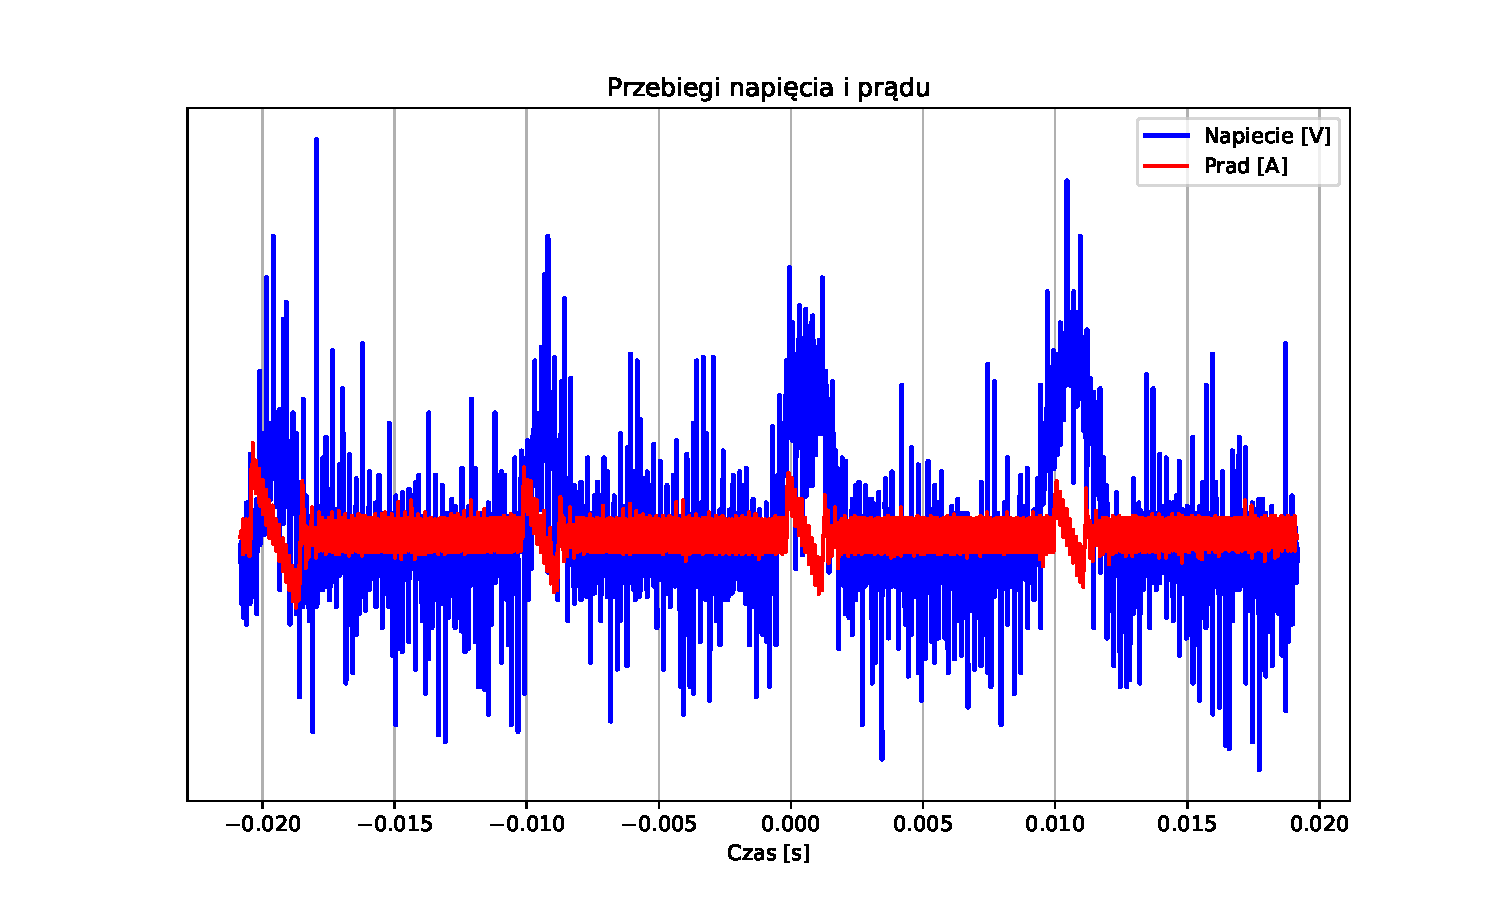
\includegraphics[width=0.8\textwidth]{aun1_dml_obciazenie_weak.pdf}
\caption{Przebieg napiecia oraz pradu na stanowisku Unidrive przy malym obciazeniu}
\end{figure}

\begin{figure}[H]
\centering
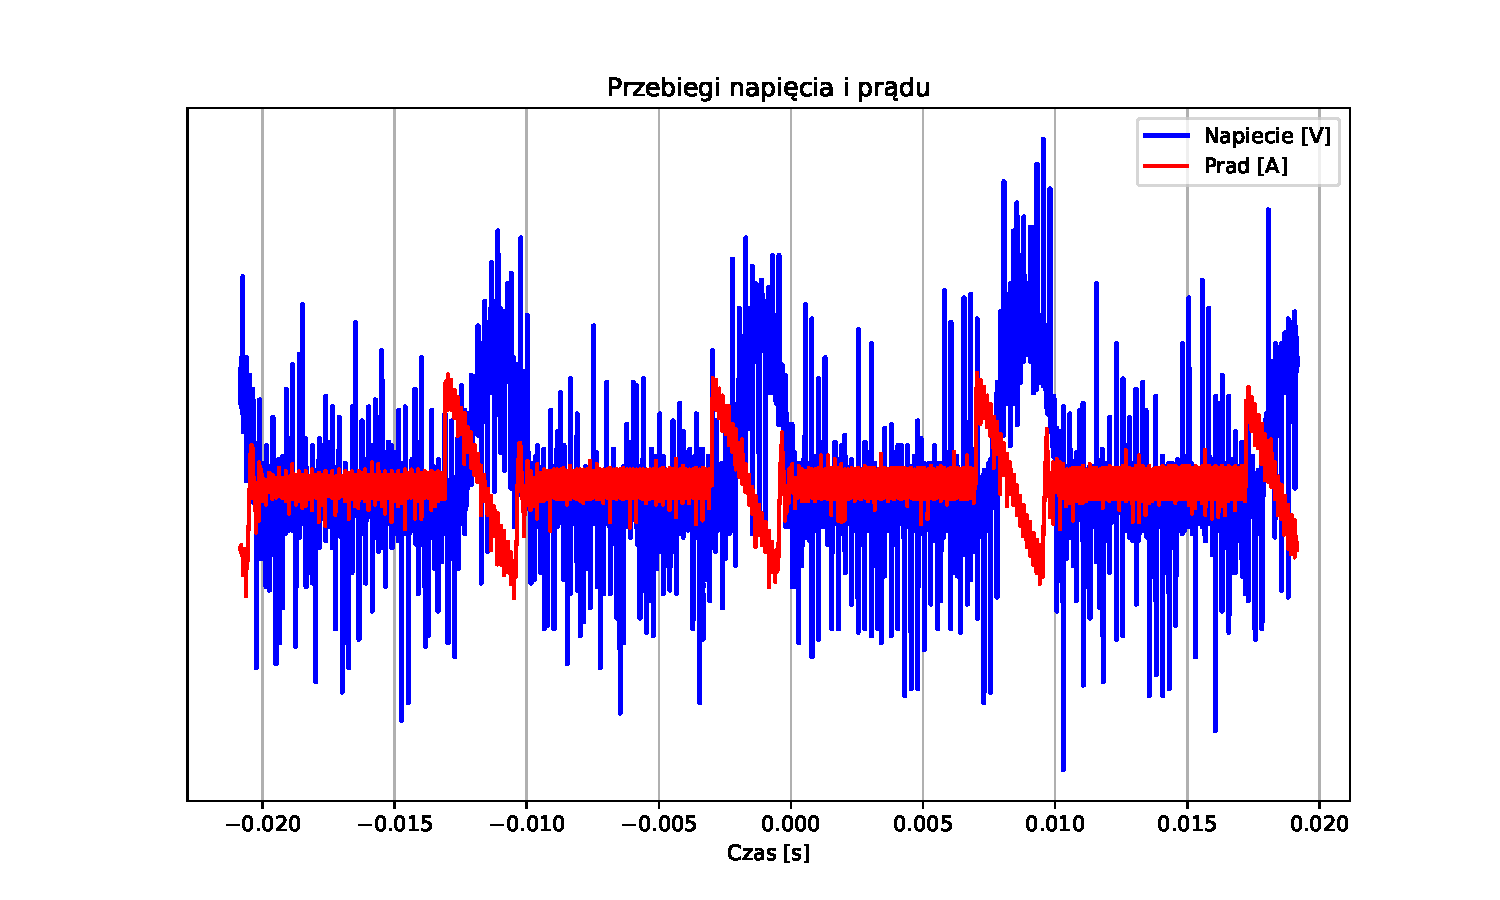
\includegraphics[width=0.8\textwidth]{aun1_dml_obciazenie_medium.pdf}
\caption{Przebieg napiecia oraz pradu na stanowisku Unidrive przy srednim obciazeniu}
\end{figure}

\begin{figure}[H]
\centering
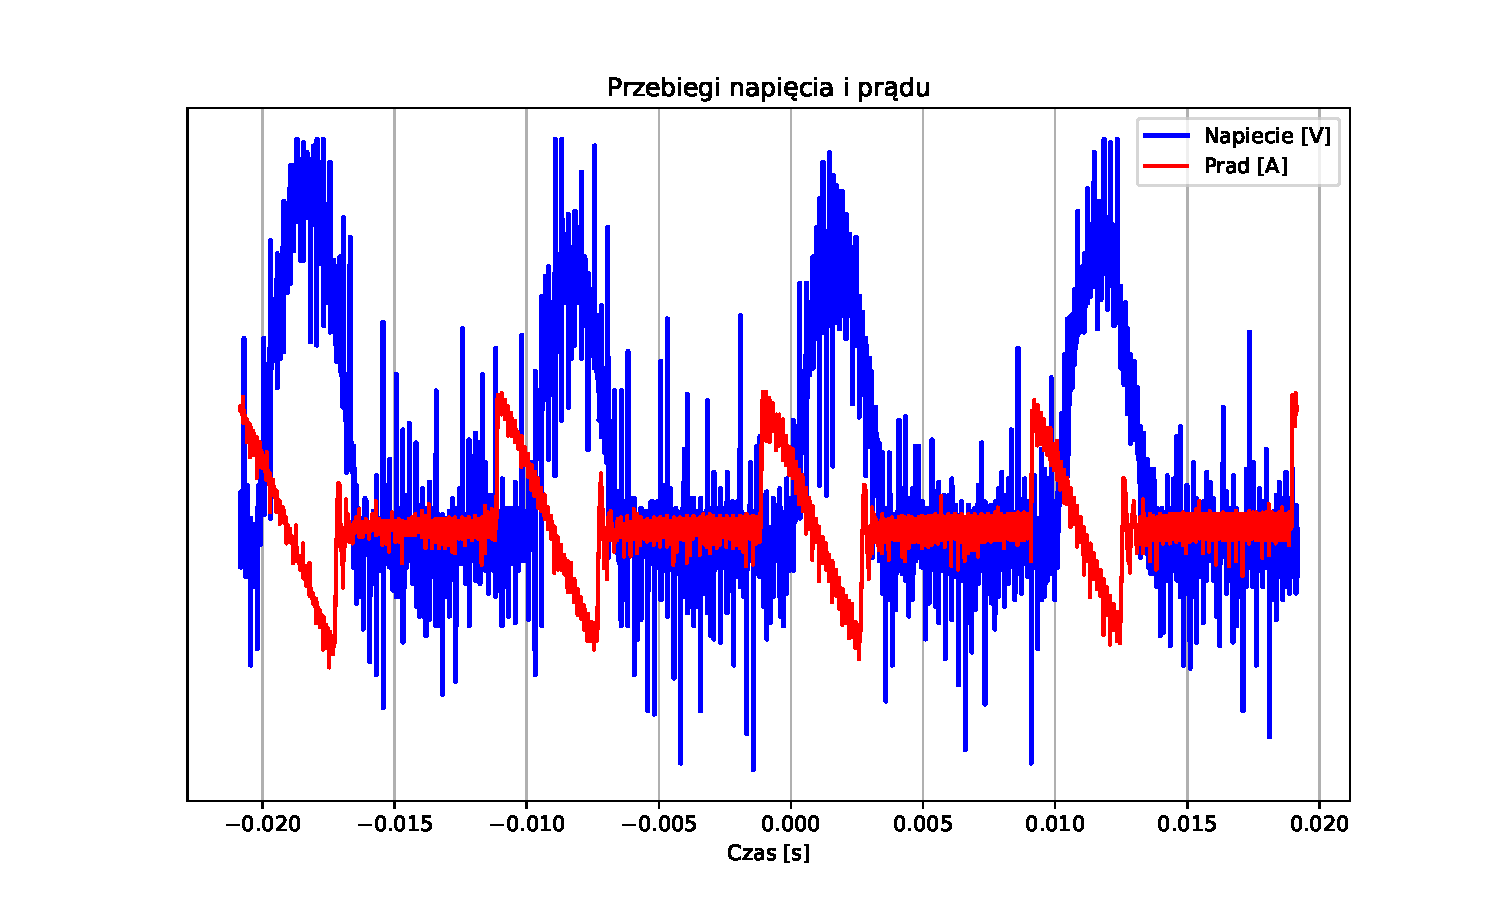
\includegraphics[width=0.8\textwidth]{aun1_dml_obciazenie_hard.pdf}
\caption{Przebieg napiecia oraz pradu na stanowisku Unidrive przy duzym obciazeniu}
\end{figure}

Tu wnioski do DML.\\

\end{document}
